\documentclass[runningheads]{llncs}

% Must pass table option to xcolor before eccv.sty loads it
\PassOptionsToPackage{table,dvipsnames}{xcolor}

% ---------------------------------------------------------------
% ECCV package
% TODO REVIEW: Insert your submission number below by replacing '*****'
% TODO FINAL: Comment out the following line for the camera-ready version
\usepackage[review,year=2026,ID=11932]{eccv}
% TODO FINAL: Un-comment the following line for the camera-ready version
%\usepackage{eccv}

% ---------------------------------------------------------------
% Other packages

\usepackage{eccvabbrv}
\usepackage{graphicx}
\usepackage{booktabs}
\usepackage[accsupp]{axessibility}

% Additional packages from our paper
%% Additional packages and commands for the paper.

% Colors for table cells
% xcolor is loaded by eccv.sty; table option is passed in main.tex
\usepackage{multirow}

\colorlet{mediumgray}{gray!60}
\colorlet{lightergray}{gray!20}
\definecolor{lightred}{RGB}{255,200,200}
\definecolor{lightgreen}{RGB}{200,255,200}
\definecolor{lightyellow}{RGB}{255,255,200}
\definecolor{lightgray}{RGB}{200,200,200}

% Inline annotations
\newcommand{\red}[1]{{\color{red}#1}}
\newcommand{\todo}[1]{{\color{red}#1}}
\newcommand{\TODO}[1]{\textbf{\color{red}[TODO: #1]}}

\usepackage{algorithm}
\usepackage{algorithmic}
\usepackage{placeins}   % \FloatBarrier for precise float placement


% ---------------------------------------------------------------
% Hyperref
% TODO FINAL: Comment out the following line for the camera-ready version
\usepackage[pagebackref,breaklinks,colorlinks,citecolor=eccvblue]{hyperref}
% TODO FINAL: Un-comment the following line for the camera-ready version
%\usepackage{hyperref}

\usepackage{orcidlink}

\begin{document}

% ---------------------------------------------------------------
\title{mmIR: Frequency-Space Inverse Rendering for 3D Millimeter-Wave Radar ADC Synthesis}

\titlerunning{mmIR: Inverse Rendering for mmWave Radar ADC Synthesis}

% TODO FINAL: Replace with your author list with ORCID
\author{First Author\inst{1} \and
Second Author\inst{1} \and
Third Author\inst{1}}

\authorrunning{F.~Author et al.}

% TODO FINAL: Replace with your institution
\institute{University, City, Country\\
\email{\{first,second,third\}@university.edu}}

\maketitle

% ---------------------------------------------------------------
% Main paper
\begin{abstract}
High-resolution 3D radar data is scarce: commodity mmWave sensors use small antenna arrays that limit angular resolution to several degrees, and existing datasets provide only 2D range--azimuth maps or sparse point clouds rather than raw ADC. Hardware scaling is expensive, synthetic-aperture scanning is impractical at fleet scale, and learned synthesis methods are bottlenecked by the very data shortage they aim to address.
%
We present mmIR, an open-source differentiable FMCW radar inverse renderer that fits a physics-based forward model to real captures and re-renders from dense virtual apertures to synthesize high-resolution 3D radar data. Using LiDAR-derived meshes as a geometric scaffold, mmIR optimizes per-vertex ITU physics materials, vertex normals, and antenna beam patterns through end-to-end automatic differentiation of a phase-coherent MIMO forward model with multi-bounce propagation, polarization, and free-space diffraction.
%
On seven outdoor ColoRadar scenes, mmIR achieves 0.63 mean Pearson correlation on range--azimuth maps versus 0.32 for Sionna-RT. Scenes trained on a cascaded imaging radar transfer to a co-located single-chip radar without re-training (0.58 correlation), and dense virtual arrays (100$\times$100 elements) produce single-frame 3D occupancy validated against LiDAR.

\keywords{Differentiable rendering \and FMCW radar \and Inverse rendering \and mmWave \and 3D reconstruction}
\end{abstract}

\section{Introduction}

\begin{figure}[t]
  \centering
  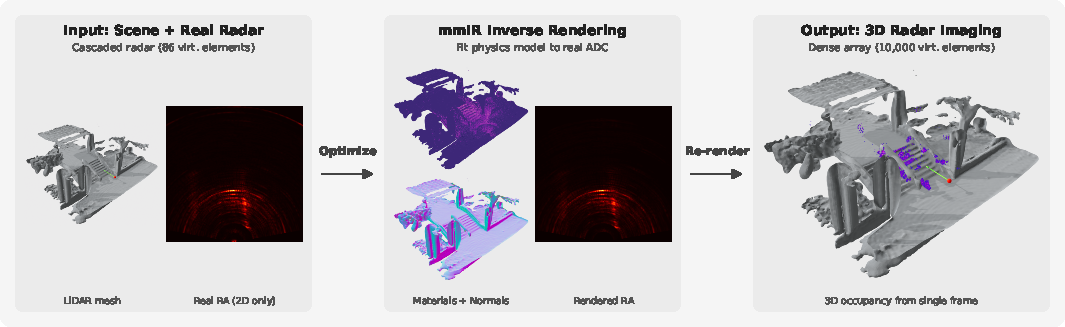
\includegraphics[width=\linewidth]{figs/teaser/teaser_v3.pdf}
  \caption{\textbf{Left:} LiDAR mesh and real 2D range--azimuth (RA) map from a commodity cascaded radar. \textbf{Center:} mmIR optimizes per-vertex materials, normals, and antenna beam patterns by fitting rendered ADC to real measurements. \textbf{Right:} The optimized scene is re-rendered from a dense 100$\times$100 virtual array for single-frame 3D occupancy detection.}
  \label{fig:teaser}
\end{figure}

Millimeter-wave (mmWave) radar penetrates fog, rain, and airborne dust~\cite{guan2020through}, measures Doppler velocity, and returns strong echoes from metals, yet it remains underutilized for 3D scene understanding. Commercial single-chip radars have only tens of antennas, limiting angular resolution to several degrees~\cite{gao2019experiments}, and their axis-biased layouts yield 2D range--azimuth (RA) slices rather than full 3D range--azimuth--elevation (RAE) volumes. Public datasets further limit access by providing only post-processed outputs (RA maps or sparse point clouds) rather than raw ADC~\cite{barnes2020oxford,caesar2020nuscenes}. The result is a shortage of high-resolution, 3D, raw FMCW ADC data: the fundamental bottleneck for learning-based radar perception. Detection, segmentation, occupancy prediction, and super-resolution all require training signal that current sensors and datasets cannot supply, and addressing this gap would enable these applications.

Existing approaches each fall short. Hardware scaling~\cite{sun2020mimo} increases cost without addressing data diversity. SAR~\cite{watts20162d,lin2023millimeter,zhang20173d} requires mechanical scanning impractical at fleet scale. Neural and Gaussian synthesis methods~\cite{mostajabi2020high,10.1145/3641519.3657510,huang2024dart,takawale2025spinr,kung2025radarsplat} are bottlenecked by the very data scarcity they aim to address: models trained on low-resolution 2D RA maps cannot recover 3D structure that was never observed.

Physics-based ray tracing (SBR) for mmWave is well established~\cite{dudek2010millimeter,sionna}, but existing pipelines are forward-only: geometry and materials must be specified \emph{a priori}, with no mechanism to calibrate against real measurements. Differentiable rendering has closed this gap for RGB~\cite{li2018differentiable, zhang2022iron}, LiDAR~\cite{kato2020differentiable}, and acoustics~\cite{jin2024diffsound}, and emerging RF methods take initial steps. Sionna RT~\cite{sionna} exposes gradients for antenna patterns and scattering coefficients but not through ray tracing itself (no geometry or normal gradients) and does not model wideband FMCW signals. Hofmann et al.~\cite{hofmann2025inverse} estimate SFCW materials but assume known geometry with single-bounce propagation, and InverTwin~\cite{chen2025invertwin} addresses multipath gradient pathologies but validates on synthetic data only. What is missing is an end-to-end differentiable FMCW renderer that can learn scene parameters from real radar captures without requiring ground-truth materials.

We present mmIR, an open-source differentiable FMCW radar inverse renderer that fits a physics-based forward model to real captures and re-renders from dense virtual apertures to synthesize high-resolution 3D radar data. Radar resolution is too coarse to reconstruct geometry directly, so we use LiDAR-derived meshes~\cite{kazhdan2006poisson} as a geometric scaffold, a practical choice given the far greater availability and resolution of LiDAR data. Inverse rendering then recovers the electromagnetic properties: mmIR optimizes per-vertex ITU physics materials (permittivity, roughness, correlation length, blend factor, slab thickness), vertex normals, and antenna beam patterns through end-to-end automatic differentiation of a phase-coherent MIMO forward model with multi-bounce propagation, polarization-aware BSDFs, specular manifold sampling~\cite{zeltner2020specular}, and free-space diffraction~\cite{steinberg2024fsd}. The pipeline also supports differentiable geometry and 6-DoF pose gradients with projective boundary sampling~\cite{zhang2023projective}, though we keep these fixed in our experiments because LiDAR-radar alignment preprocessing (Sec.~\ref{sec:supp_alignment} in the supplement) already provides accurate geometry and pose. After fitting, the optimized scene is frozen and re-rendered from arbitrarily large virtual apertures to synthesize dense, physics-consistent raw ADC (Fig.~\ref{fig:teaser}), enabling downstream applications such as 3D occupancy detection, radar super-resolution, and synthetic training data generation that would otherwise require prohibitively large physical arrays.

On seven outdoor ColoRadar~\cite{kramer2022coloradar} scenes, mmIR achieves 0.63 mean Pearson RA correlation versus 0.32 for Sionna-RT. We demonstrate cross-sensor transfer: scenes trained on a cascaded imaging radar (12TX$\times$16RX, 86 virtual elements) produce valid ADC for a co-located single-chip radar (3TX$\times$4RX, 12 virtual elements) without re-training (0.58 correlation), providing evidence that the optimized scenes capture transferable physics rather than sensor-specific patterns. We further show single-frame 3D occupancy detection from dense virtual arrays (100TX$\times$100RX) validated against LiDAR. Our contributions are:

\begin{enumerate}
\item To the best of our knowledge, the first open-source, end-to-end differentiable inverse renderer for wideband FMCW radar, enabling joint optimization of per-vertex materials, normals, and antenna patterns directly from real radar captures, with support for multi-bounce propagation, specular manifold sampling, polarization-aware BSDFs, free-space diffraction, and differentiable geometry and pose gradients with projective boundary sampling.
\item A virtual-aperture re-rendering framework that synthesizes high-resolution 3D raw ADC from fitted scenes via arbitrarily large synthetic arrays, enabling 2D-to-3D lifting and 3D occupancy detection.
\item Cross-sensor transfer validation on real COTS radar, demonstrating that scenes optimized on one sensor generalize to a different configuration without re-training.
\end{enumerate}

\subsection{Scope}
\label{sec:scope}

The primary goal of mmIR is high-quality ADC radar data synthesis: by fitting a differentiable forward model to real radar captures on real LiDAR-derived geometry, mmIR produces dense, physics-consistent raw ADC that would otherwise require expensive hardware arrays to acquire. We envision practitioners using optimized scenes to generate large-scale datasets for training downstream perception models (detection, segmentation, occupancy prediction) without additional data collection. We validate on real measurements from commercial off-the-shelf (COTS) radars, specifically the Texas Instruments MMWCAS-RF-EVM cascade and AWR1843 single-chip sensors, demonstrate cross-sensor transfer, and show that the synthesized data is sufficient for single-frame 3D occupancy detection from dense virtual arrays (Sec.~\ref{sec:3d_occupancy}). Our experimental evaluation compares against open-source, physics-based ray-tracing inverse rendering methods (Table~\ref{tab:polarization_comparison}), ensuring reproducibility and a like-for-like comparison of explicit forward models.

\begin{table}[t]
\centering
\caption{Feature comparison of physics-based differentiable radar renderers. Signal: ADC\,=\,raw FMCW, CIR\,=\,channel impulse response, IF\,=\,intermediate-frequency phasors. Multi-b.\,=\,multi-bounce; Diffr.\,=\,edge diffraction; Polar.\,=\,polarization; Geom.\,=\,differentiable geometry; Norm.\,=\,differentiable normals; Mat.\,=\,physics material model; Per-vtx\,=\,per-vertex materials; Bound.\,$\nabla$\,=\,boundary gradients; Real\,=\,validated on real data. Checkmarks denote supported pipeline capabilities; see Sec.~\ref{sec:supp_training} in the supplement for which parameters are active in our experiments.}
\label{tab:polarization_comparison}
\small
\setlength{\tabcolsep}{3pt}
\renewcommand{\arraystretch}{1.1}
\resizebox{\linewidth}{!}{
\begin{tabular}{|l|c|c|c|c|c|c|c|c|c|c|c|c|c|c|}
\hline
\rowcolor{mediumgray}
\textbf{Method} &
\textbf{Open} &
\textbf{Repr.} &
\textbf{Signal} &
\textbf{Multi-b.} &
\textbf{Diffr.} &
\textbf{Polar.} &
\textbf{Geom.} &
\textbf{Norm.} &
\textbf{Mat.} &
\textbf{Pose} &
\textbf{Beam} &
\textbf{Per-vtx} &
\textbf{Bound. $\nabla$} &
\textbf{Real} \\
\hline
\cellcolor{lightergray}Sionna RT~\cite{sionna} &
\cellcolor{lightgreen}$\checkmark$ &
\cellcolor{lightgreen}Mesh &
\cellcolor{lightyellow}CIR &
\cellcolor{lightgreen}$\checkmark$ &
\cellcolor{lightgreen}$\checkmark$ &
\cellcolor{lightgreen}$\checkmark$ &
\cellcolor{lightred}-- &
\cellcolor{lightred}-- &
\cellcolor{lightyellow}No BRDF &
\cellcolor{lightgreen}$\checkmark$ &
\cellcolor{lightred}-- &
\cellcolor{lightred}-- &
\cellcolor{lightred}-- &
\cellcolor{lightred}-- \\
\hline
\cellcolor{lightergray}SFCW Inv.~\cite{hofmann2025inverse} &
\cellcolor{lightgreen}$\checkmark$ &
\cellcolor{lightgreen}Mesh &
\cellcolor{lightyellow}IF &
\cellcolor{lightred}-- &
\cellcolor{lightred}-- &
\cellcolor{lightgreen}$\checkmark$ &
\cellcolor{lightred}-- &
\cellcolor{lightyellow}Shading &
\cellcolor{lightgreen}$\checkmark$ &
\cellcolor{lightyellow}Pos. &
\cellcolor{lightred}-- &
\cellcolor{lightgreen}$\checkmark$ &
\cellcolor{lightred}-- &
\cellcolor{lightgreen}$\checkmark$ \\
\hline
\cellcolor{lightergray}InverTwin~\cite{chen2025invertwin} &
\cellcolor{lightred}-- &
\cellcolor{lightgreen}Mesh &
\cellcolor{lightyellow}CIR &
\cellcolor{lightgreen}$\checkmark$ &
\cellcolor{lightgreen}$\checkmark$ &
\cellcolor{lightred}-- &
\cellcolor{lightgreen}$\checkmark$ &
\cellcolor{lightred}-- &
\cellcolor{lightyellow}No BRDF &
\cellcolor{lightgreen}$\checkmark$ &
\cellcolor{lightred}-- &
\cellcolor{lightred}-- &
\cellcolor{lightgreen}$\checkmark$ &
\cellcolor{lightgreen}$\checkmark$ \\
\hline
\cellcolor{lightergray}mmIR (Ours) &
\cellcolor{lightgreen}$\checkmark$ &
\cellcolor{lightgreen}Mesh &
\cellcolor{lightgreen}ADC &
\cellcolor{lightgreen}$\checkmark$ &
\cellcolor{lightgreen}$\checkmark$ &
\cellcolor{lightgreen}$\checkmark$ &
\cellcolor{lightgreen}$\checkmark$ &
\cellcolor{lightgreen}$\checkmark$ &
\cellcolor{lightgreen}$\checkmark$ &
\cellcolor{lightgreen}$\checkmark$ &
\cellcolor{lightgreen}$\checkmark$ &
\cellcolor{lightgreen}$\checkmark$ &
\cellcolor{lightgreen}$\checkmark$ &
\cellcolor{lightgreen}$\checkmark$ \\
\hline
\end{tabular}
}
\end{table}

\section{Related Works}

\textbf{Differentiable rendering beyond optics.}
Differentiable rendering couples explicit scene parameterizations with gradient-based optimization to recover geometry, materials, and sensor parameters~\cite{veach1995optimally, veach1998robust, ramamoorthi2007first, gargallo2007minimizing}. Core advances include analytic inverse rendering and MC estimator reparameterizations~\cite{li2018differentiable,loubet2019reparameterizing, bangaru2020unbiased}, as well as practical path tracing systems and neural/hybrid representations~\cite{mildenhall2021nerf, 10.1145/3550469.3555397, zhang2022iron, 10.1145/3355089.3356498, jakob2022dr, bangaru2023slang}. These methods operate almost exclusively in the optical regime. In RF, Sionna RT~\cite{sionna} propagates gradients through field coefficients and CIR computation but not through path topology: its path solver runs under gradient suspension and subsequently detaches all path geometry, so vertex positions and surface normals receive no gradients, restricting inverse rendering to quantities that enter only the CIR computation (antenna patterns, scattering coefficients, TX/RX positions). It also does not model wideband FMCW signals; Hofmann et al.~\cite{hofmann2025inverse} estimate SFCW materials but require known geometry, model only single-bounce propagation, and treat visibility as non-differentiable; and InverTwin~\cite{chen2025invertwin} addresses multipath gradient pathologies via path-space differentiation but substitutes a Gaussian kernel surrogate for radar range processing and validates on synthetic data only. mmIR bridges this gap with end-to-end AD through ray tracing itself, enabling gradients to flow through all bounces back to geometry, materials, and sensor parameters directly from raw frequency-space FMCW ADC (Table~\ref{tab:polarization_comparison}).

\begin{figure}[t]
  \centering
  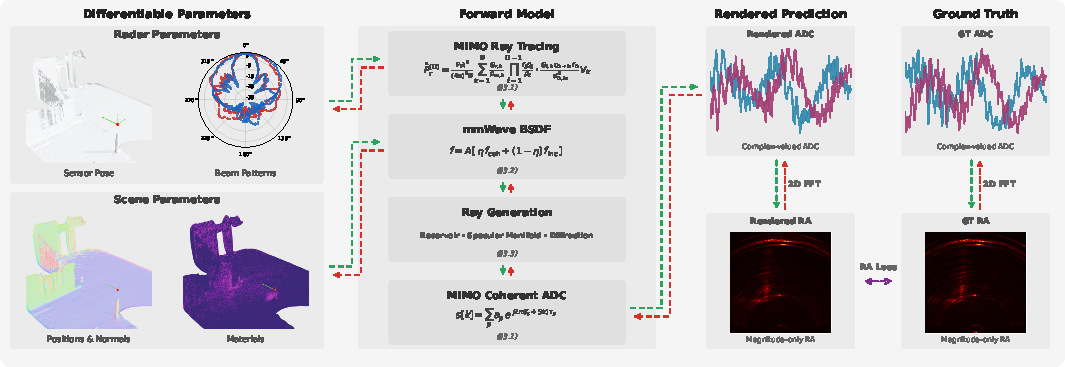
\includegraphics[width=\linewidth]{figs/pipeline/pipeline_v3.pdf}
  \caption{Overview of the mmIR pipeline. Given a LiDAR-derived mesh and initial sensor parameters, the differentiable forward model traces phase-coherent MIMO paths via multiple importance sampling over reflection and diffraction for all TX--RX pairs, then synthesizes raw FMCW ADC. End-to-end automatic differentiation through the full path (ray tracing $\to$ BSDF $\to$ phasor accumulation $\to$ ADC) enables joint optimization of per-vertex materials, geometry, normals, and 6-DoF radar pose from a range--azimuth reconstruction loss.}
  \label{fig:system}
\end{figure}

\textbf{Ray tracing for FMCW signal modeling.}
Radar simulation typically employs shooting-and-bouncing rays (SBR) to scale beyond full-wave solvers, producing path geometry and attenuation for large scenes and MIMO arrays~\cite{dudek2010millimeter}. Recent computational RF imaging further demonstrates multi-bounce physics for reconstruction on real mmWave hardware~\cite{dodds2025mito}. However, these pipelines are forward-only: scene and sensor parameters are fixed, precluding calibration against real captures. mmIR makes SBR-style FMCW rendering fully differentiable, exposing gradients w.r.t.\ mesh geometry, per-vertex materials, radar pose, and antenna patterns to close the sim-to-real gap.

\textbf{Neural and Gaussian methods for radar data synthesis.}
Neural fields have been adapted to radar across modalities: SAR/ISAR shape reconstruction~\cite{lei2024sar,deng2024isar}, FMCW occupancy and Doppler recovery~\cite{takawale2025spinr,huang2024dart}, frequency-space response synthesis~\cite{10.1145/3641519.3657510,zhang2025rf4d}, and multi-modal fusion with RGB/LiDAR~\cite{rafidashti2025neuradar,lu2024newrf}. RadarSplat~\cite{kung2025radarsplat} provides a Gaussian splatting~\cite{3dgs} alternative for range--azimuth rendering. These methods learn opaque, sensor-specific representations: DART~\cite{huang2024dart} discards phase entirely (magnitude-only range--Doppler supervision), none expose physically interpretable material parameters, and none model multi-bounce propagation, polarization, or diffraction. Moreover, methods that render post-processed images directly must learn to reproduce FFT point-spread artifacts (sidelobes, windowing); by rendering raw ADC, mmIR applies identical FFT processing to both rendered and measured data, cleanly decoupling scene physics from signal processing. mmIR maintains an explicit mesh with per-vertex ITU materials and polarization-aware BSDFs, enabling joint scene--sensor calibration and re-rendering from arbitrary virtual apertures for 3D imaging.

% \section{Related Works}

% \subsection{Differentiable Rendering}

% Classical differentiable rendering couples explicit or implicit 3D scene representations with gradient-based optimization to recover geometry, materials, and camera parameters from images~\cite{veach1995optimally, veach1998robust, ramamoorthi2007first, gargallo2007minimizing}. Early work focused on analytic inverse rendering and reparameterizations of Monte Carlo estimators~\cite{li2018differentiable,loubet2019reparameterizing, bangaru2020unbiased}, while more recent methods combine NeRF-style volumetric representations with differentiable path tracing~\cite{mildenhall2021nerf, 10.1145/3550469.3555397, zhang2022iron} and practical systems such as Mitsuba 2~\cite{10.1145/3355089.3356498}, Dr.Jit~\cite{jakob2022dr}, and Slang.d~\cite{bangaru2023slang} for general-purpose inverse rendering. These approaches operate almost exclusively in the optical regime and assume narrowband sensors with simple projective geometry. Sionna RT tackles this by extending differentiable ray tracing to the RF domain for wireless communications, exposing gradients with respect to antenna patterns, materials, and deployment parameters~\cite{sionna}, but it targets link-level channel metrics rather than high-resolution 3D imaging and does not model FMCW-specific signal generation or raw ADC samples. Hofmann et al.  introduce an SFCW radar inverse renderer that estimates material parameters from near-field measurements given known geometry~\cite{hofmann2025inverse}, and InverTwin proposes a differentiable RF digital twin that addresses gradient pathologies from multipath and path creation/destruction at the level of channel responses~\cite{chen2025invertwin}. mmIR is complementary to these efforts. We specialize differentiable rendering to wideband FMCW radar and operate directly in frequency-space ADC coordinates, with a multi-bounce, polarization-aware, diffraction-enabled forward model. Table~\ref{tab:polarization_comparison} compares and evaluates our proposed method against three other radar inverse renderers.

% % Need better version of this: Unlike RF digital twins that optimize path-wise channel coefficients, mmIR jointly optimizes b LiDAR-registered mesh geometry, per-vertex materials, radar pose, and per-antenna patterns from real FMCW captures and then re-uses the optimized scene as a generator for wide virtual apertures.

% \subsection{Ray Tracing for Radar Data Synthesis}

% Physics-based radar simulation has a long history in microwave imaging and remote sensing. Full-wave solvers that directly discretize Maxwell’s equations offer high accuracy but are too expensive for large scenes or repeated optimization. To improve scalability, many works adopt high-frequency approximations such as shooting-and-bouncing rays (SBR), modeling propagation via geometric optics plus heuristic diffraction terms. Recent simulators for automotive radar build on these ideas to support large MIMO arrays and digital-twin environments, combining CAD models with ray tracing and simplified material models for specular and diffuse scattering. For FMCW radar, Dudek et al.\ derive a frequency-domain signal model that connects transmitted chirps, propagation paths, and sampled baseband signals, providing a bridge between ray-tracing outputs and the ADC domain used in hardware~\cite{dudek2010millimeter}. In parallel, computational RF imaging systems such as MITO demonstrate that carefully designed multi-bounce imaging setups can recover geometry through occluders using optimization on real mmWave hardware~\cite{dodds2025mito}. These frameworks are typically used in a purely forward or task-specific manner: geometry and materials are fixed, and simulators generate synthetic data without gradient feedback, or reconstruction pipelines are tied to a particular sensor. mmIR builds directly on SBR-style multi-bounce ray tracing and FMCW signal modeling, but turns them into a general-purpose differentiable inverse renderer. We integrate polarization-aware BRDFs and edge diffraction into an FMCW frequency-space forward model and expose gradients with respect to mesh geometry, per-vertex materials, vertex normals, radar pose, and per-antenna patterns, allowing us to optimize and fit raw frequency-space ADC radar data to real captures, and then re-render as wide synthetic arrays for 3D mmWave reconstruction.

% \subsection{Neural Methods for Radar Data Synthesis}

% Neural radiance fields and related implicit representations have transformed view synthesis and 3D reconstruction in the optical domain~\cite{mildenhall2021nerf,kerbl20233d}, and extensions to LiDAR and multi-sensor fusion have shown benefits from incorporating explicit range measurements. A growing body of work adapts these ideas to radar. SAR-NeRF and ISAR-NeRF formulate NeRF-style inverse problems for SAR and ISAR, respectively, reconstructing voxel grids or target shapes from radar images using differentiable SAR imaging equations~\cite{lei2024sar,deng2024isar}. SpINR couple an implicit neural volume with a differentiable frequency-domain FMCW forward model to recover dense occupancy from raw radar data~\cite{takawale2025spinr}. For automotive-style FMCW radar, DART learns an implicit Doppler tomography representation from range–Doppler data for novel-view synthesis and multipath analysis~\cite{huang2024dart}. Radar Fields synthesizes raw radar data directly in frequency space, learning a neural field that map 3D coordinates and view direction to complex FMCW responses and occupancy for scanning trajectories~\cite{10.1145/3641519.3657510}. RF4D extends neural fields to dynamic outdoor driving scenes by treating time as an additional dimension~\cite{zhang2025rf4d}. NeuRadar and NeWRF train NeRF-style models on sparse automotive radar point clouds jointly with RGB/LiDAR to enable multi-modal novel view synthesis and radar simulation in adverse weather~\cite{rafidashti2025neuradar,lu2024newrf}. Rather than learning a purely neural volume, we start from a LiDAR-registered mesh with physically interpretable per-vertex materials and normals, and fit this scene directly to raw frequency-domain FMCW data consistent with radar physics. This allows us to jointly calibrate scene and sensor parameters, maintain compatibility with graphics BRDF models, and then render synthetic wide-aperture arrays for 3D reconstruction, instead of only learning a forward neural mapper from radar signals to occupancy or images.

% \subsection{Gaussian Splatting for Radar Data Synthesis}

% Gaussian splatting offers an explicit, real-time alternative to NeRF by representing scenes as a set of anisotropic 3D Gaussians optimized for view synthesis~\cite{3dgs}. In the optical domain, Gaussian splatting achieves high-fidelity, real-time rendering on large-scale datasets and has been extended to panoramic cameras and RGB-D streams. These methods typically assume photometric radiance accumulation and camera-based sensor models. Recent work adapts Gaussian splatting to radar imaging. RadarSplat~\cite{kung2025radarsplat} introduces a Gaussian representation tailored to FMCW radar, attaching complex-valued scattering amplitudes and radar-specific attributes to each Gaussian and rendering frequency-space or range–azimuth images from scanning trajectories using a radar equation–based forward model. mmIR differs from radar Gaussian splatting in both representation and goal. We do not learn Gaussian primitives; instead, we maintain an explicit mesh-based scene with polarization-aware BRDFs and per-antenna gain models, and treat radar synthesis as differentiable FMCW rendering. This lets us directly optimize geometry, materials, and sensor parameters against real frequency-domain data and then re-render from arbitrary virtual apertures, while remaining tightly anchored to the underlying radar physics.


\section{Methods}
\label{sec:methods}

We model radar sensing as a forward rendering problem (Fig.~\ref{fig:system}): trace multi-bounce rays through a scene, evaluate surface interactions via a physically-based mmWave BSDF, and accumulate phase-coherent paths into raw FMCW ADC samples that can be directly compared against real captures. Sec.~\ref{sec:forward_model} derives the forward model from the bistatic radar equation through multi-bounce Monte Carlo estimation to ADC synthesis; Sec.~\ref{sec:bsdf} defines the mmWave BSDF governing surface interactions; Sec.~\ref{sec:sampling} describes ray generation strategies; and Sec.~\ref{sec:optimization} formulates the differentiable inverse rendering pipeline.

Our inputs are synchronized radar--LiDAR data from ColoRadar~\cite{kramer2022coloradar}. LiDAR frames are aggregated into a triangle mesh via screened Poisson reconstruction~\cite{kazhdan2006poisson}, and a GPU-accelerated coarse-to-fine alignment corrects residual sensor misregistration (Sec.~\ref{sec:supp_preprocessing}--\ref{sec:supp_alignment} in the supplement). FMCW signal and TDM-MIMO imaging derivations are in the supplement (Sec.~\ref{sec:rationale}--\ref{sec:tdm_mimo_imaging}).

\subsection{Forward Model}
\label{sec:forward_model}

Our forward model is grounded in the bistatic radar equation. For a single TX--RX pair observing a point target at surface point $\mathbf{x}$ with normal $\mathbf{n}$, at distances $d_t$, $d_r$ from transmitter and receiver, the received power $P_r$ is:
\begin{equation}
    P_r
    =
    \frac{P_t\, G_t\, G_r\, \lambda^2\, \sigma}{(4\pi)^3\, d_t^2\, d_r^2},
    \label{eq:radar_bistatic}
\end{equation}
where $P_t$ is transmit power, $G_t$, $G_r$ are directional antenna gains, $\lambda$ is wavelength, and $\sigma$ is the bistatic radar cross-section. Replacing the point-target RCS with a spatially varying BSDF $f(\boldsymbol{\omega}_t, \mathbf{x}, \boldsymbol{\omega}_r)$, where $\boldsymbol{\omega}_t$ and $\boldsymbol{\omega}_r$ are unit directions toward the transmitter and receiver, and converting from surface area element $dA_x$ to receiver solid angle via $d\omega_r = (c_r / d_r^2)\,dA_x$ with $c_r = \max(0, \mathbf{n} \cdot \boldsymbol{\omega}_r)$ (derivation in the supplement, Sec.~\ref{sec:supp_mc_derivation}), the total received power integrated over the receiver hemisphere $\Omega_{rx}$ becomes:
\begin{equation}
    P_r
    =
    \frac{P_t\,\lambda^2}{(4\pi)^2}
    \int_{\Omega_{rx}}
    \frac{
    G_t(\boldsymbol{\omega}_t)\,G_r(\boldsymbol{\omega}_r)\,
    f(\boldsymbol{\omega}_t, \mathbf{x}, \boldsymbol{\omega}_r)\,
    c_t\, V
    }{
    d_t^2
    }
    \, d\omega_r,
    \label{eq:radar_solid_angle}
\end{equation}
where $c_t = \max(0, \mathbf{n} \cdot \boldsymbol{\omega}_t)$ is the cosine factor and $V \in \{0,1\}$ is visibility. This solid-angle formulation directly motivates RX-centric sampling: trace rays from the receiver, intersect the scene, and evaluate the integrand with a deterministic connection to the transmitter.

For multi-bounce propagation with path depth $D$ and interaction points $\mathbf{x}_1, \ldots, \mathbf{x}_D$, each stochastically sampled segment contributes a BSDF-over-PDF ratio and geometric coupling. Given $N$ Monte Carlo samples, the unbiased estimator is (derivation in the supplement, Sec.~\ref{sec:supp_mc_derivation}):
\begin{equation}
    \hat{P}_r^{(D)}
    =
    \frac{P_t\,\lambda^2}{(4\pi)^2}\,
    \frac{1}{N}\sum_{k=1}^{N}
    \frac{G_{r,k}}{\rho_{rx,k}}
    \prod_{\ell=1}^{D{-}1}
    \frac{f_\ell\, \mathcal{G}_\ell}{\rho_\ell}
    \;\cdot\;
    \frac{G_{t,k}\, c_{D{\to}tx}\, f_D}{d_{D,tx}^2}
    \, V_k,
    \label{eq:mc_multibounce}
\end{equation}
where $\mathcal{G}_\ell = c_{\ell{\to}\ell{+}1}\, c_{\ell{+}1{\to}\ell}\,/\,d_{\ell,\ell{+}1}^2$ is the geometric coupling between consecutive bounces, with $c_{\ell{\to}\ell{+}1} = \max(0, \mathbf{n}_\ell \cdot \boldsymbol{\omega}_{\ell{\to}\ell{+}1})$ the cosine factor at bounce $\ell$ toward bounce $\ell{+}1$ and $d_{\ell,\ell{+}1}$ the distance between them. The BSDF at each bounce is $f_\ell = f(\boldsymbol{\omega}_{\ell-1}, \mathbf{x}_\ell, \boldsymbol{\omega}_{\ell+1})$ (Sec.~\ref{sec:bsdf}), which decomposes each surface interaction into slab transmission, coherent specular reflection, incoherent diffuse scattering, and edge diffraction. The final term connects deterministically to the transmitter: $c_{D{\to}tx}$ is the cosine factor at $\mathbf{x}_D$ toward the TX and $d_{D,tx}$ is their distance. The sampling PDFs $\rho_\ell$ are determined by the ray generation strategies in Sec.~\ref{sec:sampling}. The single-bounce case ($D{=}1$) reduces to $G_t\,G_r\,c_t\,f\,V\,/\,(d_t^2\,\rho_{rx})$, and we use Russian roulette~\cite{veach1998robust} for unbiased path termination.

The MC estimator provides a complex amplitude for each traced path. To synthesize raw FMCW ADC, each path $p$ for TX $i$ and RX $j$ contributes a phase-delayed chirp sample using the complex baseband form (Sec.~\ref{sec:supp_fmcw}--\ref{sec:supp_iq} in the supplement):
\begin{equation}
    s_{ij}^{(p)}[k]
    =
    a_{ij}^{(p)}
    \exp\!\Big(j\, 2\pi (f_c + S t_k)\,\tau_{ij}^{(p)} \Big),
    \label{eq:path_adc}
\end{equation}
where $k$ indexes fast-time ADC samples at times $t_k$, $j$ is the imaginary unit, $\tau_{ij}^{(p)} = R_{ij}^{(p)}/c$ is the round-trip delay for total path length $R_{ij}^{(p)}$ at speed of light $c$, $f_c$ is the carrier frequency, $S$ is the chirp slope, and $a_{ij}^{(p)} \in \mathbb{C}$ aggregates the MC throughput from Eq.~\eqref{eq:mc_multibounce}: antenna gains, BSDF evaluations, geometric coupling, and spreading losses. The rendered ADC sums coherently over all paths: $s_{ij}[k] = \sum_p s_{ij}^{(p)}[k]$.

Equations~\eqref{eq:radar_bistatic}--\eqref{eq:path_adc} describe a single TX--RX pair. In a MIMO array, each pair is evaluated independently through the same forward model; however, coherent MIMO imaging via FFT~\cite{9658500} requires exact relative phase across all pairs, so independent MC samples per receiver would corrupt this. Following the MIMO ray reuse strategy of Sch{\"u}{\ss}ler et al.~\cite{9533181}, we share path topology across all TX--RX pairs: a single set of interaction points is found from shared seeds, then evaluated for all pairs by vectorizing only the TX$\rightarrow\mathbf{x}_1$ and $\mathbf{x}_D\rightarrow$RX legs. Each pair produces unique amplitudes and phases but shares bounce topology, preserving MIMO coherence while reducing cost from $\mathcal{O}(N_\mathrm{TX} \cdot N)$ to $\mathcal{O}(N)$.

\subsection{Physically-Based mmWave BSDF}
\label{sec:bsdf}

The BSDF $f$ appearing in the MC estimator (Eq.~\eqref{eq:mc_multibounce}) governs how electromagnetic energy is redistributed at each surface interaction. We model it using ITU-R P.2040 recommendations for mmWave propagation~\cite{itu_p2040}, inspired by the coherent spatially varying BSDF (CSVBSDF) formulation of Wei et al.~\cite{wei2024csvbsdf}. Each mesh vertex stores six physically interpretable material parameters: real and imaginary relative permittivity $(\varepsilon_r', \varepsilon_r'')$, RMS surface roughness $\sigma_h$, correlation length $l_c$, a KA/SPM blend factor $\tau$, and slab thickness $d$. At each ray--triangle intersection, parameters are barycentric-interpolated from the three triangle vertices ($\mathbf{m}_i \in \mathbb{R}^6$), ensuring $C^0$-continuous material fields with gradients flowing to all three vertices.

The BSDF decomposes into coherent and incoherent components via the Rayleigh roughness factor~\cite{beckmann1963scattering} $\eta = \exp(-(2k\sigma_h\cos\theta_t)^2)$, $k=2\pi/\lambda$, where $\theta_t$ is the incidence angle between $\boldsymbol{\omega}_t$ and the surface normal:
\begin{equation}
    f = A(\boldsymbol{\omega}_t)\;\Big[\eta\,f_\mathrm{coh} + (1-\eta)\,f_\mathrm{inc}\Big],
    \label{eq:bsdf_full}
\end{equation}
where $A(\boldsymbol{\omega}_t) \in [0,1]$ is the slab Fresnel energy gate. The lobe decompositions are:
\begin{align}
    f_\mathrm{coh} &= \tau\, f_\mathrm{KA} + (1{-}\tau)\, f_\mathrm{SPM}, \label{eq:bsdf_coh} \\
    f_\mathrm{inc} &= \gamma\, f_\mathrm{dir} + (1{-}\gamma)\, f_\mathrm{broad}, \label{eq:bsdf_inc}
\end{align}
where $\tau$ is a learnable KA/SPM blend and $\gamma$ is a roughness-dependent sigmoid. The coherent lobes are: $f_\mathrm{KA}$, a GGX microfacet specular lobe~\cite{walter2007microfacet} with roughness $\alpha = \sqrt{4\pi\sigma_h/\lambda}$; and $f_\mathrm{SPM}$, a von Mises--Fisher (vMF) distribution centered on the specular direction with concentration $\kappa = \sqrt{l_c/\lambda}\,/\,(1 + 3\sigma_h/l_c)$~\cite{ulaby2019microwave}. The incoherent lobes are: $f_\mathrm{dir}$, a broader vMF lobe; and $f_\mathrm{broad}$, Lambertian. The energy gate $A(\boldsymbol{\omega}_t)$ uses an ITU-R P.2040 slab model with thickness $d$ and complex permittivity $\varepsilon_r = \varepsilon_r' - j\varepsilon_r''$, capturing multiple internal reflections rather than single-interface Fresnel.

The Fresnel coefficients in the energy gate also determine polarization state, which we maintain throughout path tracing using a local $s/p$ basis. At each interaction, the complex Fresnel coefficients derived from learnable permittivity update both amplitude and phase of the $s$ and $p$ field components~\cite{born2013principles}. Between bounces, the polarization basis is transported deterministically to preserve phase consistency. The polarization-dependent energy gate is $A = f_s |r_s|^2 + f_p |r_p|^2$, where $r_s$, $r_p$ are the complex Fresnel reflection coefficients for the $s$ and $p$ polarizations and $f_s$, $f_p$ are the antenna-dependent power fractions in each polarization.

\subsection{Ray Generation}
\label{sec:sampling}

The MC estimator (Eq.~\eqref{eq:mc_multibounce}) requires sampling ray directions at each interaction. Because the mmWave BSDF (Sec.~\ref{sec:bsdf}) combines smooth diffuse, near-delta specular, and edge-diffraction components that no single sampling PDF can efficiently cover, we provide the PDFs $\rho_\ell$ via three complementary strategies combined with multiple importance sampling (MIS)~\cite{veach1995optimally} and balance heuristic weights.

\paragraph{RX-centric reservoir sampling.}
\label{sec:surface_sampling}
Because mmWave antennas are highly directional, we employ RX-centric reservoir sampling inspired by Resampled Importance Sampling (RIS)~\cite{talbot2005importance} and spatiotemporal reservoir resampling (ReSTIR)~\cite{bitterli2020spatiotemporal, lin2022generalized}. For each RX element, we sample $M$ candidate directions from a cosine-weighted hemisphere proposal centered on the RX boresight, $\rho_{rx}(\boldsymbol{\omega}) = \cos\theta / \pi$, which naturally concentrates samples within the antenna main lobe, then retain $K$ directions that successfully intersect scene geometry.

\paragraph{Specular manifold sampling.}
\label{sec:sms}
LiDAR-derived meshes contain triangles much smaller than the mmWave wavelength ($\lambda \approx 3.9$~mm). The image method (mirroring TX across the hit triangle's plane) frequently fails because the exact specular point falls outside the original triangle. We instead use Specular Manifold Sampling (SMS)~\cite{zeltner2020specular}, which solves for exact reflection points via Newton iteration on the half-vector constraint $\mathbf{C}(\mathbf{x}) = [\mathbf{s}{\cdot}\mathbf{h},\; \mathbf{t}{\cdot}\mathbf{h}]^\top = \mathbf{0}$, where $\mathbf{s},\mathbf{t}$ are surface tangents and $\mathbf{h}$ is the half-vector. After each Newton step, re-projection onto the mesh via ray tracing allows the solver to cross triangle boundaries, producing exact specular paths with deterministic Fresnel weights.

We extend SMS for radar inverse rendering with: GPU-vectorized Newton iteration via DrJit~\cite{jakob2022dr}, Implicit Function Theorem (IFT) gradient support that stores the Jacobian inverse at convergence for backpropagation through vertex positions, and multi-bounce specular chain solving via a block-tridiagonal algorithm.

\paragraph{Free-space diffraction BSDF.}
\label{sec:fsd}
Unlike the Uniform Theory of Diffraction (UTD), which requires explicit edge detection and separate ray classes, the free-space diffraction (FSD) BSDF~\cite{steinberg2024fsd} formulates edge diffraction as a standard scattering distribution compatible with path tracing. At each intersection, the FSD BSDF projects nearby triangles onto a virtual screen, identifies boundary edges, and evaluates closed-form Fraunhofer diffraction integrals. A fraction $\beta$ of reflected energy is redirected into importance-sampleable diffracted lobes.

We extend FSD for mmWave radar with: (i) material-dependent edge opacity via Fresnel reflectance from learnable permittivity; (ii) Jones polarization tracking through diffracted paths for MIMO phase coherence; and (iii) edge suppression filters that reject artifacts from noisy LiDAR tessellation.

\subsection{Differentiable Optimization}
\label{sec:optimization}

We optimize per-vertex ITU physics materials ($6 \times N_v$ parameters with sigmoid/exponential reparameterizations for physical bounds), per-vertex normals $\mathbf{N} \in \mathbb{R}^{N_v \times 3}$, and antenna beam patterns. The pipeline additionally supports differentiable vertex positions and 6-DoF radar pose, but we keep these fixed in our experiments: our coarse-to-fine LiDAR-radar alignment (Sec.~\ref{sec:supp_alignment} in the supplement) already provides sub-centimeter translational and sub-degree rotational accuracy, so the remaining sim-to-real gap is dominated by material and scattering properties rather than geometric misregistration. Initialization uses ITU-R P.2040 reference values for common materials (concrete, glass, metal). Details on bounds, learning rates, and schedules are in the supplement (Sec.~\ref{sec:supp_training}).

The entire forward model (Secs.~\ref{sec:forward_model}--\ref{sec:sampling}) executes inside a single DrJit~\cite{jakob2022dr} computation graph with automatic differentiation. Gradients flow from $\mathcal{L}$ through the ADC, per-path phasors, BSDF evaluations, and ray--triangle intersections back to all learnable parameters in a single backward pass. At silhouette edges where visibility changes discontinuously, projective boundary gradient sampling~\cite{zhang2023projective} corrects gradient bias for vertex positions and pose when these are enabled.

\paragraph{Loss function.}
We minimize a range--azimuth reconstruction loss on min--max normalized magnitudes:
\begin{equation}
    \mathcal{L}_\mathrm{RA}
    =
    \frac{1}{|\Gamma|}
    \sum_{(r,a)\in\Gamma}
    \big\lVert \widetilde{\mathrm{RA}}_\mathrm{render}(r,a) - \widetilde{\mathrm{RA}}_\mathrm{gt}(r,a) \big\rVert_2^2,
    \label{eq:ra_loss}
\end{equation}
where $\Gamma$ is the set of range--azimuth bins, $\widetilde{\mathrm{RA}} = (\mathrm{RA} - \min\mathrm{RA}) / (\max\mathrm{RA} - \min\mathrm{RA})$ denotes min--max normalization, and RA maps are obtained via the TDM-MIMO FFT pipeline~\cite{9658500}. Operating directly on linear magnitudes gives uniform gradient weighting across the dynamic range, avoiding the gradient imbalance that log-compression introduces near the noise floor. The total objective is $\mathcal{L} = \mathcal{L}_\mathrm{RA} + \lambda_\mathrm{geom}\mathcal{L}_\mathrm{geom}$, where $\lambda_\mathrm{geom}$ is a regularization weight and $\mathcal{L}_\mathrm{geom}$ enforces geometric smoothness via Laplacian regularization on vertex normals and positions. After convergence, we freeze optimized parameters and re-render from dense virtual apertures to synthesize 3D radar data (Sec.~\ref{sec:3d_occupancy}).
%% Phase sensitivity and inference -- commented out for now:
%At 77~GHz ($\lambda \approx 3.9$~mm), phase varies as $\phi \propto R/\lambda$, so micrometer-scale path-length changes induce large phase swings, creating a highly oscillatory loss landscape~\cite{chen2025invertwin}. We address this with per-parameter-group RMS gradient clipping and linear learning rate warmup (Sec.~\ref{sec:phase_sensitivity_loss_landscape}). At inference, we freeze optimized parameters and re-render from dense virtual apertures to synthesize 3D radar data (Sec.~\ref{sec:3d_occupancy}).

\section{Experiments}

\begin{figure}[t]
  \centering
  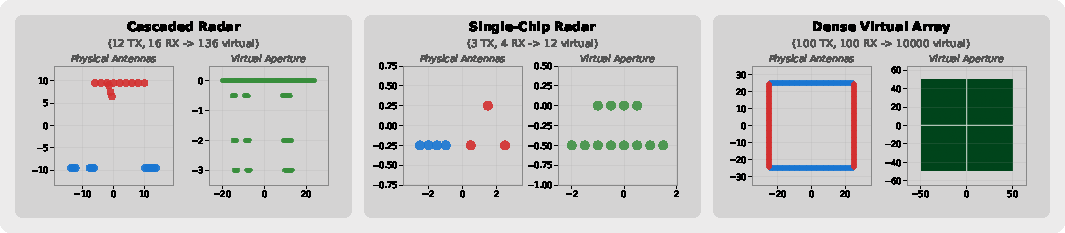
\includegraphics[width=\linewidth]{figs/antenna_layouts.pdf}
  \caption{Antenna configurations used in our evaluation. Left: cascaded MMWCAS-RF-EVM (12TX$\times$16RX $\to$ 86 unique azimuth virtual elements; Sec.~\ref{sec:supp_range_angle_resolution} in the supplement) used for training. Center: single-chip AWR1843 (3TX$\times$4RX $\to$ 12 virtual elements) used for cross-sensor transfer. Right: dense virtual array (100TX$\times$100RX $\to$ 10{,}000 virtual elements) used for 3D inference. Top row: physical TX (red) and RX (blue) positions. Bottom row: virtual aperture (TX$+$RX convolution).}
  \label{fig:antenna_layouts}
\end{figure}

We evaluate mmIR on seven diverse outdoor scenes from the ColoRadar dataset~\cite{kramer2022coloradar}, which provides synchronized mmWave radar and LiDAR captures with raw ADC access. We design three experiments that progressively test our forward model under increasingly challenging conditions: (1)~training evaluation on the cascaded imaging radar used for optimization (12TX$\times$16RX, 86 virtual elements); (2)~cross-sensor transfer to a co-located single-chip radar (3TX$\times$4RX, 12 virtual elements) without re-training; and (3)~3D occupancy inference via a dense virtual array (100TX$\times$100RX, 10{,}000 virtual elements). Figure~\ref{fig:antenna_layouts} illustrates all three antenna configurations. Dataset details, scene geometry reconstruction, and implementation hyperparameters are provided in the supplement (Sec.~\ref{sec:supp_implementation}).

\subsection{Training Evaluation: ADC Rendering and Range--Azimuth}
\label{sec:training_ra}

% Table 1: Training RA — Per-scene results with aggregate
\begin{table}[t]
\centering
\caption{Range--azimuth (RA) and ADC training evaluation across seven outdoor scenes. mmIR is compared against Sionna-RT~\cite{sionna}. Metrics: Pearson correlation (Corr), PSNR, SSIM, RMSE, and ADC-level magnitude error. Best in \textbf{bold}.}
\label{tab:training_ra}
\resizebox{\linewidth}{!}{%
\begin{tabular}{l cc cc cc cc cc cc}
\toprule
& \multicolumn{2}{c}{RA Correlation $\uparrow$} & \multicolumn{2}{c}{RA PSNR $\uparrow$} & \multicolumn{2}{c}{RA SSIM $\uparrow$} & \multicolumn{2}{c}{RA RMSE $\downarrow$} & \multicolumn{2}{c}{ADC Log-Mag MSE $\downarrow$} & \multicolumn{2}{c}{ADC MM-Mag MSE $\downarrow$} \\
\cmidrule(lr){2-3} \cmidrule(lr){4-5} \cmidrule(lr){6-7} \cmidrule(lr){8-9} \cmidrule(lr){10-11} \cmidrule(lr){12-13}
Scene & Ours & Sionna & Ours & Sionna & Ours & Sionna & Ours & Sionna & Ours & Sionna & Ours & Sionna \\
\midrule
  S0F135 & \textbf{0.921} & 0.418 & \textbf{37.4} & 21.4 & \textbf{0.938} & 0.509 & \textbf{0.0135} & 0.0850 & \textbf{48.3271} & 244.8361 & \textbf{0.0421} & 0.0469 \\
  S0F390 & \textbf{0.936} & 0.242 & \textbf{41.0} & 23.4 & \textbf{0.937} & 0.550 & \textbf{0.0089} & 0.0674 & \textbf{5.0250} & 294.3032 & \textbf{0.0289} & 0.0417 \\
  S1F185 & \textbf{0.954} & 0.312 & \textbf{39.8} & 18.9 & \textbf{0.926} & 0.326 & \textbf{0.0102} & 0.1138 & \textbf{32.3385} & 282.6453 & \textbf{0.0398} & 0.0461 \\
  S1F438 & \textbf{0.942} & 0.346 & \textbf{37.7} & 19.9 & \textbf{0.926} & 0.401 & \textbf{0.0130} & 0.1008 & \textbf{32.5274} & 288.9782 & \textbf{0.0369} & 0.0435 \\
  S2F105 & \textbf{0.887} & 0.188 & \textbf{34.6} & 28.7 & \textbf{0.894} & 0.724 & \textbf{0.0185} & 0.0367 & \textbf{23.5161} & 244.9075 & 0.0498 & \textbf{0.0481} \\
  S2F160 & \textbf{0.864} & 0.370 & \textbf{34.0} & 22.4 & \textbf{0.789} & 0.519 & \textbf{0.0200} & 0.0763 & \textbf{27.6683} & 275.3327 & \textbf{0.0444} & 0.0461 \\
  S2F300 & \textbf{0.930} & 0.388 & \textbf{38.7} & 21.3 & \textbf{0.906} & 0.512 & \textbf{0.0117} & 0.0858 & \textbf{30.0014} & 247.1371 & \textbf{0.0370} & 0.0543 \\
\midrule
  Mean & \textbf{0.919$\pm$0.030} & 0.324$\pm$0.076 & \textbf{37.6$\pm$2.4} & 22.3$\pm$3.0 & \textbf{0.902$\pm$0.049} & 0.506$\pm$0.115 & \textbf{0.0137$\pm$0.0038} & 0.0808$\pm$0.0229 & \textbf{28.4863$\pm$11.9698} & 268.3057$\pm$20.3703 & \textbf{0.0399$\pm$0.0061} & 0.0467$\pm$0.0037 \\
\bottomrule
\end{tabular}
}
\end{table}

\begin{figure}[t]
  \centering
  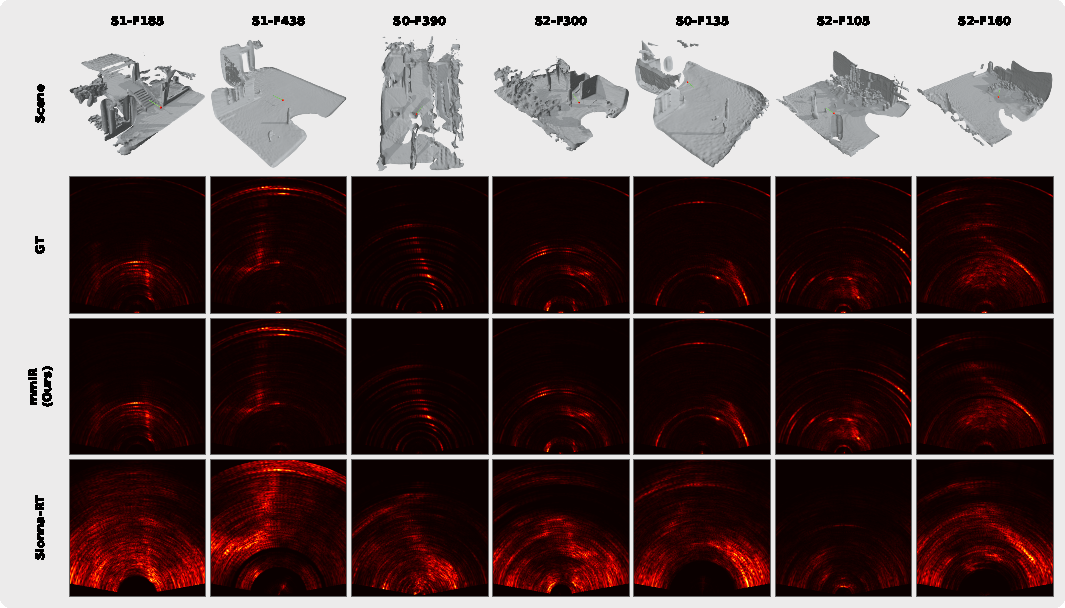
\includegraphics[width=\linewidth]{figs/training_ra/training_single_v2.pdf}
  \caption{Qualitative range--azimuth (RA) comparison across all seven training scenes, sorted by Pearson correlation (highest first). Each column shows one scene. Rows, top to bottom: scene mesh with radar position (red sphere) and boresight direction (green arrow); ground-truth RA; mmIR (ours); Sionna-RT baseline. Horizontal axis: cross-range (m); vertical axis: range (m). mmIR captures the dominant scatterer structure and multipath returns across all scenes, while Sionna-RT produces weaker, less spatially accurate responses.}
  \label{fig:eval_ra}
\end{figure}

We compare rendered and measured range--azimuth (RA) maps on the cascaded radar used for optimization. Table~\ref{tab:training_ra} reports Pearson correlation, PSNR, SSIM, RMSE, and ADC-level magnitude metrics across all seven scenes, with Sionna-RT~\cite{sionna} as baseline. Evaluating in the RA domain implicitly validates phase accuracy: the azimuth FFT converts relative phase differences across virtual elements into angular information, so any systematic phase error (per-element bias, incorrect path-length scaling, or incoherent phasor accumulation) would smear or shift targets in the angular domain, degrading all RA metrics. Absolute phase is not meaningful in practice, as it depends on user-configurable initial phase, oscillator drift, and phase noise; these common-mode offsets appear in the DC term of the spatial FFT and are dropped during processing.

mmIR achieves a mean Pearson correlation of \textbf{0.919}, substantially outperforming Sionna-RT (0.324). Table~\ref{tab:training_ra} quantifies this gap across all metrics; Figure~\ref{fig:eval_ra} provides the corresponding qualitative comparison, sorted by correlation. mmIR reproduces both the dominant scatterer locations and the diffuse multipath structure present in the ground truth, whereas Sionna-RT produces attenuated responses with spatially misaligned features.

Three architectural differences drive this gap. First, mmIR's physically-based BSDF with six per-vertex learnable parameters captures spatially varying reflectance that Sionna-RT's per-object scattering model cannot represent; this is most evident in geometrically complex scenes (S1-F438, S0-F135) where mixed-material surfaces dominate the radar response. Second, mmIR jointly optimizes surface normals and antenna beam patterns, parameters entirely outside Sionna-RT's optimization scope, correcting both surface orientation errors inherited from noisy LiDAR tessellation and systematic antenna gain biases. Third, Sionna-RT's path solver executes outside the AD graph: ray tracing runs under gradient suspension and all path geometry is subsequently detached, so while material gradients propagate through field coefficients at each bounce, the path topology itself is frozen and no gradients reach vertex positions or normals, and a material change at one surface cannot redirect subsequent bounces. mmIR places the entire forward model inside a single computation graph, enabling end-to-end gradient flow from the loss through ADC synthesis, phasor accumulation, BSDF evaluation, and ray--triangle intersections. The weakest scene, S2F160 (0.864), shows that even challenging geometries with complex multipath achieve high correlation. mmIR substantially outperforms the baseline on every scene, indicating that the richer parameter space and deeper gradient flow consistently improve fit quality.

\subsection{Radar Transfer Evaluation}
\label{sec:radar_transfer}

% Table 2: Radar Transfer — Per-scene results with aggregate
\begin{table}[t]
\centering
\caption{Cross-sensor transfer evaluation. Scene parameters optimized on the cascaded radar (12TX$\times$16RX, 86 unique azimuth virtual elements) are frozen and used to render ADC for the co-located single-chip radar (3TX$\times$4RX, 12 virtual elements) without re-training. Best in \textbf{bold}.}
\label{tab:radar_transfer}
\resizebox{\linewidth}{!}{%
\begin{tabular}{l cc cc cc cc cc cc}
\toprule
& \multicolumn{2}{c}{RA Correlation $\uparrow$} & \multicolumn{2}{c}{RA PSNR $\uparrow$} & \multicolumn{2}{c}{RA SSIM $\uparrow$} & \multicolumn{2}{c}{RA RMSE $\downarrow$} & \multicolumn{2}{c}{ADC Log-Mag MSE $\downarrow$} & \multicolumn{2}{c}{ADC MM-Mag MSE $\downarrow$} \\
\cmidrule(lr){2-3} \cmidrule(lr){4-5} \cmidrule(lr){6-7} \cmidrule(lr){8-9} \cmidrule(lr){10-11} \cmidrule(lr){12-13}
Scene & Ours & Bench. & Ours & Bench. & Ours & Bench. & Ours & Bench. & Ours & Bench. & Ours & Bench. \\
\midrule
  S0F135 & \textbf{0.533} & 0.002 & \textbf{25.6} & 17.8 & \textbf{0.505} & 0.464 & \textbf{0.0524} & 0.1283 & \textbf{10.9639} & 301.4341 & 0.2194 & \textbf{0.0668} \\
  S0F390 & \textbf{0.464} & 0.328 & 21.2 & \textbf{24.2} & 0.529 & \textbf{0.566} & 0.0873 & \textbf{0.0619} & \textbf{12.9644} & 331.2549 & \textbf{0.0630} & 0.0840 \\
  S1F185 & \textbf{0.567} & 0.136 & \textbf{22.4} & 20.1 & 0.422 & \textbf{0.480} & \textbf{0.0759} & 0.0990 & \textbf{0.5754} & 324.8441 & 0.1993 & \textbf{0.0771} \\
  S1F438 & \textbf{0.684} & 0.079 & \textbf{23.2} & 13.5 & \textbf{0.674} & 0.202 & \textbf{0.0694} & 0.2119 & \textbf{21.8672} & 348.0237 & 0.1507 & \textbf{0.0662} \\
  S2F105 & \textbf{0.608} & 0.084 & \textbf{24.7} & 22.8 & 0.609 & \textbf{0.690} & \textbf{0.0583} & 0.0721 & \textbf{3.4458} & 289.7929 & 0.1959 & \textbf{0.1068} \\
  S2F160 & \textbf{0.276} & 0.159 & \textbf{19.3} & 18.3 & \textbf{0.493} & 0.463 & \textbf{0.1085} & 0.1219 & \textbf{20.1530} & 338.1699 & 0.0893 & \textbf{0.0798} \\
  S2F300 & \textbf{0.745} & 0.008 & \textbf{27.2} & 23.6 & \textbf{0.468} & 0.412 & \textbf{0.0434} & 0.0661 & \textbf{7.7226} & 287.9379 & 0.1074 & \textbf{0.0948} \\
\midrule
  Mean & \textbf{0.554$\pm$0.143} & 0.114$\pm$0.103 & \textbf{23.4$\pm$2.5} & 20.0$\pm$3.6 & \textbf{0.529$\pm$0.080} & 0.468$\pm$0.138 & \textbf{0.0707$\pm$0.0206} & 0.1087$\pm$0.0488 & \textbf{11.0989$\pm$7.3886} & 317.3511$\pm$22.3659 & 0.1464$\pm$0.0565 & \textbf{0.0822$\pm$0.0136} \\
\bottomrule
\end{tabular}
}
\end{table}

A central claim of physics-based inverse rendering is that the optimized scene captures true physical properties, not sensor-specific patterns. We validate this by \emph{cross-sensor transfer}: the scene parameters trained on the cascaded radar (12TX $\times$ 16RX, 86 virtual elements) are frozen and used to render ADC for the single-chip radar (3TX $\times$ 4RX, 12 virtual elements) that shares the same physical mounting (Fig.~\ref{fig:antenna_layouts}). We apply the same rigid-body alignment transformation learned during cascaded training to the single-chip configuration and render forward-only.

This experiment tests whether our inverse renderer has learned transferable scene physics rather than memorizing the training sensor's idiosyncrasies. Table~\ref{tab:radar_transfer} shows that mmIR achieves a mean transfer correlation of \textbf{0.554}, outperforming Sionna-RT (0.114), demonstrating that the learned materials generalize across sensor configurations.

\subsection{Inference: 3D Occupancy via Dense Virtual Array}
\label{sec:3d_occupancy}

\begin{table}[t]
\centering
\caption{3D occupancy evaluation against LiDAR ground truth. Baseline: ColoRadar-provided 3D point cloud from the cascaded radar's near-1D virtual aperture, where elevation is synthesized by extruding range--azimuth detections along the vertical axis due to minimal elevation resolution. Ours: dense virtual array (100TX$\times$100RX) with full 2D aperture enabling range--azimuth--elevation (RAE) imaging. Occupancy metrics use KD-tree nearest neighbors ($\tau{=}0.5$\,m). Best in \textbf{bold}.}
\label{tab:3d_occupancy}
\resizebox{\linewidth}{!}{%
\begin{tabular}{l cc cc cc cc cc cc}
\toprule
& \multicolumn{2}{c}{Precision $\uparrow$} & \multicolumn{2}{c}{Recall $\uparrow$} & \multicolumn{2}{c}{F1 $\uparrow$} & \multicolumn{2}{c}{Accuracy $\uparrow$} & \multicolumn{2}{c}{RMSE $\downarrow$} & \multicolumn{2}{c}{R-CD $\downarrow$} \\
\cmidrule(lr){2-3} \cmidrule(lr){4-5} \cmidrule(lr){6-7} \cmidrule(lr){8-9} \cmidrule(lr){10-11} \cmidrule(lr){12-13}
Scene & Ours & ColoR & Ours & ColoR & Ours & ColoR & Ours & ColoR & Ours & ColoR & Ours & ColoR \\
\midrule
  S0F135 & 0.077 & \textbf{0.223} & 0.018 & \textbf{0.054} & 0.029 & \textbf{0.087} & 0.044 & \textbf{0.057} & \textbf{2.324} & 3.302 & 0.248 & \textbf{0.228} \\
  S0F390 & \textbf{0.481} & 0.045 & \textbf{0.110} & 0.014 & \textbf{0.179} & 0.021 & \textbf{0.212} & 0.017 & \textbf{2.692} & 2.745 & 0.216 & \textbf{0.207} \\
  S1F185 & \textbf{0.997} & 0.483 & \textbf{0.566} & 0.082 & \textbf{0.722} & 0.141 & \textbf{0.703} & 0.103 & \textbf{0.909} & 2.380 & \textbf{0.067} & 0.236 \\
  S1F438 & \textbf{0.633} & 0.433 & \textbf{0.265} & 0.117 & \textbf{0.373} & 0.185 & \textbf{0.362} & 0.131 & \textbf{1.511} & 3.339 & \textbf{0.116} & 0.268 \\
  S2F105 & \textbf{0.771} & 0.154 & \textbf{0.162} & 0.025 & \textbf{0.268} & 0.044 & \textbf{0.340} & 0.029 & \textbf{1.099} & 3.402 & \textbf{0.113} & 0.282 \\
  S2F160 & \textbf{0.516} & 0.383 & \textbf{0.177} & 0.165 & \textbf{0.264} & 0.231 & \textbf{0.257} & 0.183 & 1.917 & \textbf{1.611} & 0.146 & \textbf{0.118} \\
  S2F300 & \textbf{0.850} & 0.508 & \textbf{0.501} & 0.122 & \textbf{0.630} & 0.197 & \textbf{0.601} & 0.130 & \textbf{1.040} & 1.643 & \textbf{0.083} & 0.118 \\
\midrule
  Mean & \textbf{0.618$\pm$0.278} & 0.319$\pm$0.165 & \textbf{0.257$\pm$0.189} & 0.083$\pm$0.051 & \textbf{0.352$\pm$0.228} & 0.129$\pm$0.075 & \textbf{0.360$\pm$0.210} & 0.093$\pm$0.056 & \textbf{1.642$\pm$0.638} & 2.632$\pm$0.721 & \textbf{0.141$\pm$0.062} & 0.208$\pm$0.061 \\
\bottomrule
\end{tabular}
}
\end{table}

\begin{figure}[t]
  \centering
  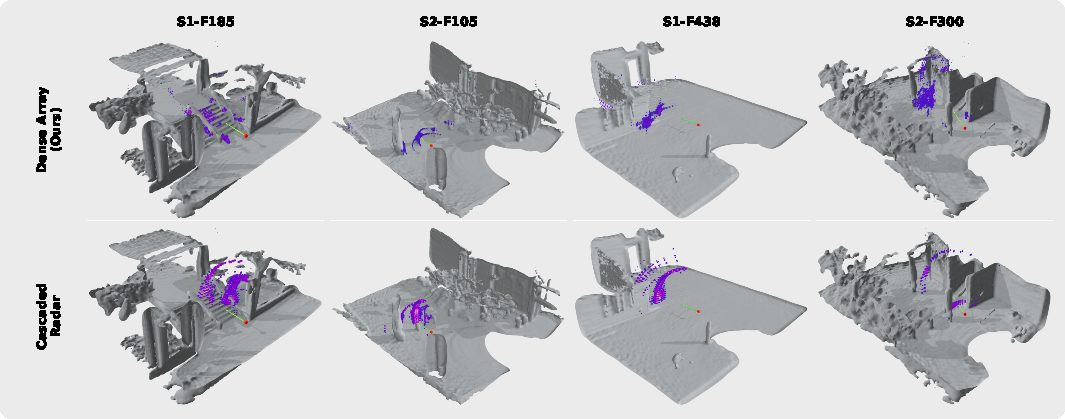
\includegraphics[width=\linewidth]{figs/test_3d/test_3d_v1.pdf}
  \caption{Single-frame 3D occupancy comparison overlaid on the LiDAR mesh. Top row: mmIR dense virtual array (100$\times$100 elements, uniform $\lambda/2$ spacing) with full 2D aperture enabling range--azimuth--elevation (RAE) imaging, thresholded at the 99.9th intensity percentile. Bottom row: ColoRadar-provided 3D point cloud from the cascaded radar's near-1D virtual aperture, which resolves only range--azimuth and extrudes detections along elevation, producing vertically smeared structure. Red sphere: radar position; green arrow: boresight direction.}
  \label{fig:3d_single_frame_comparison}
\end{figure}

After training, we freeze the optimized scene parameters and re-render from a dense virtual array (100TX $\times$ 100RX, 10,000 virtual elements with $\lambda/2$ spacing) inspired by the Rohde \& Schwarz QAR50~\cite{wirth2024maroon} (Fig.~\ref{fig:antenna_layouts}, right). We convert synthesized ADC into a 3D tensor via Range--Azimuth--Elevation (RAE) FFT and extract a sparse radar point cloud by thresholding at the 99.9th intensity percentile. Following~\cite{kung2025radarsplat}, we use single-bounce propagation at test time for the dense array.

We evaluate against LiDAR after radar-guided filtering: (1) filtering by the dense array's 0~dB beam limits, (2) projecting LiDAR points onto the radar polar voxel grid, and (3) retaining only points where radar normalized intensity $\geq 0.1$. Occupancy metrics use KD-tree nearest neighbors with $\tau=0.5$~m threshold; geometric fidelity is measured via RMSE and Relative Chamfer Distance (R-CD). Table~\ref{tab:3d_occupancy} shows substantial variation driven by radar visibility: scenes with multiple surfaces within the field-of-view achieve strong reconstruction (S1F185: Precision=0.997, R-CD=0.067), while open scenes with ground planes nearly parallel to boresight show degraded recall as specular energy is directed away from receivers. Additional qualitative analysis, quantitative ablation, and runtime results are in the supplement (Sec.~\ref{sec:supp_qualitative}).

\section{Conclusion}

We introduced mmIR, a differentiable inverse-rendering framework that fits scene and sensor parameters directly from raw FMCW ADC. By combining end-to-end automatic differentiation through phase-coherent MIMO path accumulation with ITU physics-based per-vertex materials, mmIR optimizes materials, normals, and beam patterns from real radar captures. On seven outdoor scenes, mmIR achieves 0.63 mean Pearson correlation on range--azimuth maps, substantially outperforming Sionna-RT (0.32). After fitting, the optimized scene produces sensor-realistic ADC from dense virtual apertures for 3D occupancy detection and scene reconstruction, validated against LiDAR. We further validate cross-sensor generalization by transferring trained scenes to a different radar configuration. This opens a path toward physics-grounded radar sensing pipelines, including calibration, radar-aware 3D reconstruction, and joint multi-modal optimization.

\textbf{Limitations and future work.} mmIR is bottlenecked by mesh quality: the LiDAR-to-mesh reconstruction pipeline sets a ceiling on rendered ADC realism, and the inverse rendering task is sensitive to LiDAR-radar alignment for both cascade and single-chip configurations. Our prototype further assumes static scenes and surface-only interactions (no transmission, refraction, or volumetric scattering), models diffraction at single-bounce interactions only, and does not account for Doppler phase from ego-motion. Although our pipeline supports differentiable vertex positions and pose, we found that at 77~GHz ($\lambda \approx 3.9$~mm), sub-millimeter vertex shifts induce large phase changes, making geometry and pose gradients unstable under Monte Carlo estimation with current sample budgets. Shape-from-radar, where geometry is directly recovered from radar measurements, remains a compelling goal but will likely require dense multi-view supervision and regularization strategies beyond what single-frame RA fitting provides. Natural extensions include higher-fidelity meshing, robust alignment, temporally coherent Doppler modeling, multi-bounce diffraction, and richer propagation effects. We discuss these limitations in detail in the supplement (Sec.~\ref{sec:limitations}). Scaling to jointly optimize radar with other sensors and learning priors over radar-consistent materials are promising directions for robust autonomous perception.


% ---------------------------------------------------------------
% Supplementary (appended after references for review)
\clearpage
\appendix
\section*{Supplementary Material}
\setcounter{section}{0}
\renewcommand{\thesection}{\Alph{section}}
\section{TDM MIMO FMCW Theory}
\label{sec:rationale}

This section provides the signal-processing foundations that underpin our differentiable renderer, included for readers whose background is primarily in rendering or vision rather than radar.
Sec.~\ref{sec:supp_fmcw} derives the FMCW beat signal that the renderer must synthesize per traced path.
Sec.~\ref{sec:supp_iq} explains IQ demodulation, which determines why the renderer outputs \emph{complex}-valued ADC samples.
Sec.~\ref{sec:tdm_mimo_imaging} shows how these ADC samples are transformed into the 2D range--azimuth and 3D range--azimuth--elevation images used in our training loss (Eq.~\ref{eq:ra_loss}) and evaluation metrics.
Sec.~\ref{sec:supp_mc_derivation}--\ref{sec:supp_power_to_adc} derive the Monte Carlo estimator (main paper Eq.~3) and the power-to-ADC conversion that closes the forward model.
Readers familiar with FMCW radar may skip directly to Sec.~\ref{sec:supp_implementation}.

\subsection{FMCW Formulation}
\label{sec:supp_fmcw}

We summarize the standard FMCW signal model following~\cite{skolnik2001introduction,dudek2010millimeter}. FMCW radars emit a linearly frequency-modulated chirp into the scene,
\begin{equation}
    s(t) = A_s \cos\!\left(2\pi f_c t + \pi K t^2 \right), 
\end{equation}
for $\qquad 0 < t < T_c,$ and receive a delayed echo
\begin{equation}
    u(t) = A_r \cos\!\left(2\pi f_c (t-\tau) + \pi K (t-\tau)^2 \right), 
\end{equation}
for $\qquad \tau < t < T_c$, where $K$ is the chirp slope, $f_c$ is the start frequency, $T_c$ is the chirp duration, and $\tau = 2 d(t)/c$ is the round-trip delay for a target at range $d$ and wave propagation speed $c$. The total swept bandwidth is
\begin{equation}
    B = f_{\max} - f_{\min} = (f_c + K T_c) - f_c = K T_c.
\end{equation}

When the received chirp is mixed with the (still transmitting) chirp and low-pass filtered, the resulting real-valued beat signal is
\begin{equation}
    m_{\mathrm{R}}(t) \approx A_m 
    \cos\!\left(2\pi K \tau\, t + 2\pi f_c \tau - \pi K \tau^2\right),
    \label{eq:real_beat}
\end{equation}
for $\qquad \tau < t < T_c,$ where $A_m$ subsumes constant amplitude factors. The beat frequency is
\begin{equation}
    f_{\mathrm{IF}} = K \tau = \frac{2 K d}{c},
\end{equation}
and the range-dependent phase is dominated by
\begin{equation}
    \phi(t) \approx 2\pi f_c \tau = 4\pi \frac{d}{\lambda},
\end{equation}
with carrier wavelength $\lambda = c/f_c$. The small quadratic term $\pi K \tau^2$ is typically negligible for automotive-range targets ($K\tau^2 \ll f_c\tau$).

\begin{figure}[t]
  \centering
  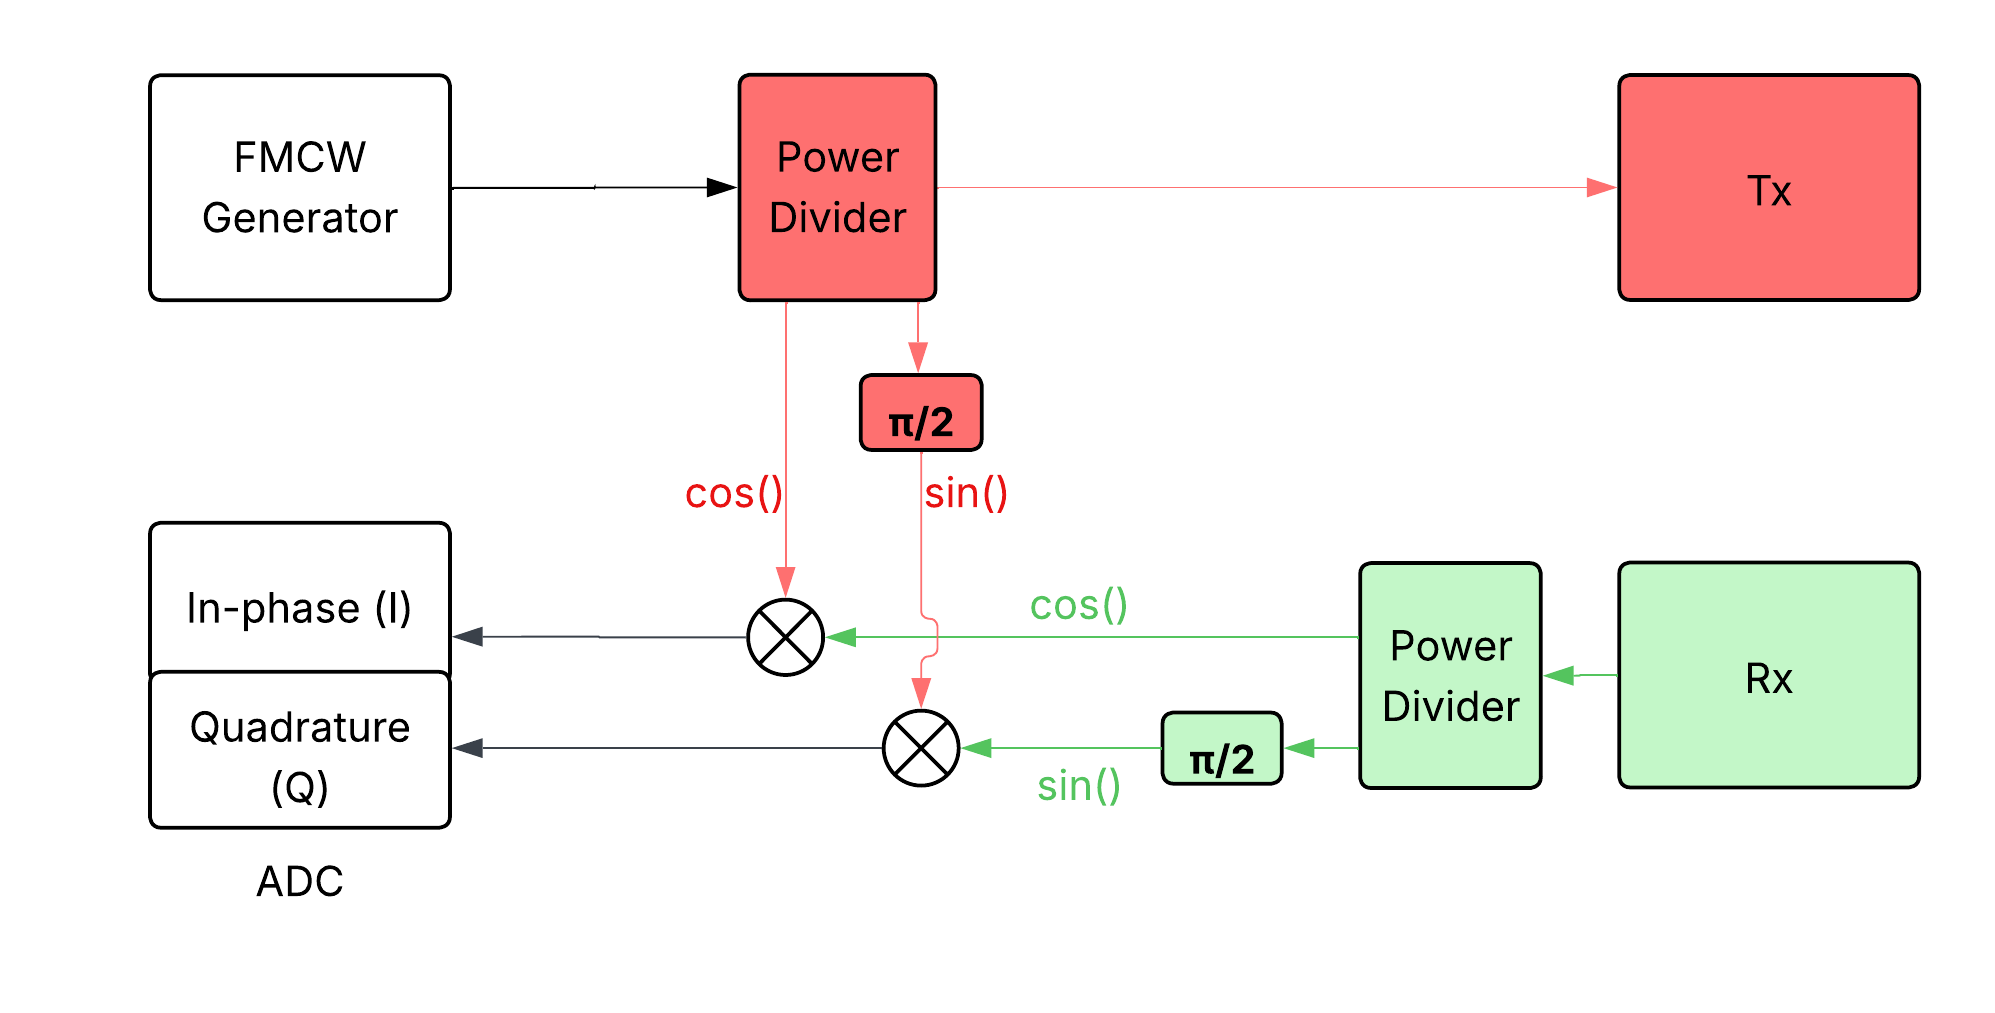
\includegraphics[width=\linewidth]{figs/IQ_demodulation.png}
  \caption{Block diagram of IQ demodulation in FMCW radar. The received echo is mixed with in-phase (I) and quadrature (Q) copies of the transmit chirp and low-pass filtered, producing complex baseband samples that preserve both amplitude and phase for downstream range and angle processing.}
  \label{fig:iq_demod}
\end{figure}

\subsection{IQ Demodulation for Complex Baseband ADC}
\label{sec:supp_iq}

In practice, the RF front-end uses IQ demodulation as shown in Fig.~\ref{fig:iq_demod}. A single real mixer would fold the symmetric RF sidebands at $\pm f_{\mathrm{IF}}$ onto the same baseband frequencies, effectively aliasing positive and negative beat frequencies onto the same baseband bins. IQ mixing instead produces a complex-valued baseband signal with a one-sided spectrum, keeping positive and negative frequencies separated, improving SNR, and yielding an unambiguous mapping between beat frequency and range~\cite{270463, alizadeh2019remote}.

A copy of the transmit chirp is routed to the local-oscillator (LO) ports of two mixers: one LO branch uses a cosine (in-phase, I) and the other a $90^\circ$-shifted sine (quadrature, Q). The received RF signal is applied to the RF port of both mixers, and each output is low-pass filtered and digitized, yielding
\begin{align}
    I(t) &\propto \cos\!\big(2\pi f_{\mathrm{IF}} t + \phi(t)\big),\\
    Q(t) &\propto \sin\!\big(2\pi f_{\mathrm{IF}} t + \phi(t)\big).
\end{align}
Interpreting these as the real and imaginary parts of a single complex baseband beat signal,
\begin{equation}
    m(t) = I(t) + j\,Q(t),
\end{equation}
is equivalent to multiplying the received RF with a complex LO and discarding the image band.

To make this analytic form explicit, we write the transmitted and received chirps using Euler’s formula following~\cite{270463}:
\begin{align}
    s(t) &= A_s \exp\!\big(j (2\pi f_c t + \pi K t^2)\big),\\
    u(t) &= A_r \exp\!\big(j [2\pi f_c (t-\tau) + \pi K (t-\tau)^2]\big).
\end{align}
Ideal IQ demodulation corresponds to mixing the received signal with the complex conjugate of the transmit signal:
\begin{equation}
    m(t) = u(t)\,s^*(t).
\end{equation}
Using the phase difference between $u(t)$ and $s(t)$, this simplifies to
\begin{align}
    m(t) 
    &= A_s A_r \exp\!\left(
        j \left[ 2\pi K \tau\, t + 2\pi f_c \tau - \pi K \tau^2 \right]
    \right) \\
    &\approx A_m \exp\!\left(
        j \left[ 2\pi f_{\mathrm{IF}} t + \phi(t) \right]
    \right),
    \label{eq:complex_baseband_continuous}
\end{align}
where again $f_{\mathrm{IF}} = K \tau = 2 K d/c$ and $\phi(t) \approx 4\pi d/\lambda$.

Finally, the ADC samples this complex baseband signal at rate $f_s$, producing discrete-time IQ data
\begin{equation}
    m[n] \approx A_m 
    \exp\!\left(
        j \left[ 2\pi f_{\mathrm{IF}} \frac{n}{f_s} + \phi[n] \right]
    \right),
    \label{eq:adc_samples}
\end{equation}
where $n$ indexes fast-time samples within a chirp and $\phi[n]$ encodes the path-length-dependent phase (and any slow motion) at the $n$-th sample. These complex ADC samples are the starting point for our subsequent MIMO imaging formulation.


\subsection{TDM MIMO for 2D and 3D Imaging}
\label{sec:tdm_mimo_imaging}

The complex ADC samples in~\eqref{eq:adc_samples} describe a single transmit--receive pair observing a single target. Modern mmWave sensors instead use multiple transmit (TX) and receive (RX) antennas arranged in an array and operate them in time-division multiplexing (TDM) mode to synthesize a larger \emph{virtual} aperture. This enables 2D and 3D spatial imaging via discrete Fourier transforms over carefully chosen dimensions of the ADC data cube, as described by~\cite{9658500}.

\paragraph{TDM MIMO data cube.}
Let $N_\text{TX}$ and $N_\text{RX}$ denote the number of physical transmitters and receivers, $N_\text{chirp}$ the number of chirps in a frame, and $N_\text{s}$ the number of fast-time ADC samples per chirp. In a TDM sequence, only one TX is active at a time. Each chirp slot is assigned to a particular transmitter, cycling through all $N_\text{TX}$ elements.

For TX element $i \in \{0,\dots,N_\text{TX}-1\}$, RX element $j \in \{0,\dots,N_\text{RX}-1\}$, chirp index $\ell \in \{0,\dots,N_\text{chirp}-1\}$, and fast-time sample index $n \in \{0,\dots,N_\text{s}-1\}$, the sampled complex beat signal can be written as
\begin{equation}
    m_{ij}[\ell,n] \approx A_{ij}[\ell]\,
    \exp\!\left(
        j\left[
            2\pi f_{\mathrm{IF}} \frac{n}{f_s}
            + \phi_{ij}[\ell]
        \right]
    \right),
    \label{eq:tdm_mimo_sample}
\end{equation}
where $f_s$~is the ADC sampling rate, $A_{ij}[\ell]$~captures path loss and BSDF/antenna gains, and the phase~$\phi_{ij}[\ell]$ contains the range phase~$4\pi d/c$ plus offsets from TX/RX array geometry and slow motion across chirps.

Stacking all $(i,j,\ell,n)$ produces a four-dimensional data block. For convenience, the TX/RX indices are often flattened into a \emph{virtual} antenna index $v \in \{0,\dots,N_\text{V}-1\}$ with $N_\text{V} = N_\text{TX} N_\text{RX}$, giving $m_v[\ell,n]$.

\paragraph{Range FFT (fast-time).}
The first processing step is a 1D FFT along fast time $n$ for each virtual channel $v$ and chirp $\ell$, which converts beat frequency to range. Before the FFT, a Hann window $w_\text{R}[n]$ is applied in fast time to suppress spectral leakage and sidelobes:
\begin{equation}
    M_v[\ell,k]
    =
    \sum_{n=0}^{N_\text{s}-1}
        w_\text{R}[n]\,
        m_v[\ell,n]\,
        \exp\!\left(
            -j \frac{2\pi}{N_\text{s}} k n
        \right),
    \label{eq:range_fft}
\end{equation}
$\qquad k = 0,\dots,N_\text{s}-1.$ Each frequency bin $k$ corresponds to a range
\begin{equation}
    R_k = \frac{c\,k}{2B},
    \label{eq:range_bin}
\end{equation}
so the magnitude $\lvert M_v[\ell,k]\rvert$ encodes the reflectivity at range $R_k$ observed by virtual channel $v$. Range estimation is therefore driven primarily by the \emph{amplitude} of the fast-time FFT, while the complex phase of $M_v[\ell,k]$ is carried forward for angle processing.

\paragraph{Angle-of-arrival from virtual array phase.}
At a fixed range bin $k$, a far-field target arriving from direction $(\theta,\varphi)$ (azimuth and elevation) produces nearly identical amplitudes across the virtual aperture but a systematic phase ramp tied to the projection of the direction vector onto each element’s position. For a 1D linear virtual array along $x$ with inter-element spacing $d_x$, the phase at element $v$ satisfies
\begin{equation}
    \phi_v(k) \approx \phi_0(k) 
    + \frac{2\pi}{\lambda}\, x_v \sin\theta,
\end{equation}
where $x_v$ is the $x$-coordinate of virtual element $v$. Taking a DFT over the virtual array index therefore steers beams in angle:
\begin{align}
\widetilde{M}[k,n_\theta]
&=
\sum_{v=0}^{N_\mathrm{V}-1}
    w_\mathrm{AZ}[v]\,
    \Big(
        \frac{1}{N_\text{chirp}}
        \sum_{\ell=0}^{N_\text{chirp}-1}
            M_v[\ell,k]
    \Big)
    \nonumber\\
&\quad\times
    \exp\!\left(
        -j \frac{2\pi}{N_\mathrm{V}} n_\theta v
    \right),
\label{eq:azimuth_fft}
\end{align}

where $w_\text{AZ}[v]$ is a spatial (e.g., Hann) window applied across the virtual aperture to reduce angular sidelobes. The bin index $n_\theta$ maps to azimuth angle via the usual array steering relation,
\begin{equation}
    \theta_{n_\theta}
    \approx \sin^{-1}\!\left(
        \frac{\lambda}{N_\text{V} d_x}\, n_\theta
    \right),
\end{equation}
assuming half-wavelength spacing and small-angle approximation. Here, the \emph{relative phase} of $M_v[\ell,k]$ across $v$ is what encodes direction-of-arrival. The FFT over $v$ converts this phase gradient into an angular spectrum. The result $\lvert \widetilde{M}[k,n_\theta]\rvert$ is a 2D range--azimuth (RA) map.

When the physical TX and RX antennas are arranged in a 2D grid, TDM MIMO produces a 2D virtual array indexed by $(v_x,v_z)$ along horizontal and vertical baselines with spacings $d_x$ and $d_z$. After the range FFT, two consecutive spatial FFTs over $v_x$ and $v_z$ yield a 3D range--azimuth--elevation (RAE) cube:
\begin{align}
\widetilde{M}_x[k,n_\theta,v_z]
&=
\sum_{v_x} w_\text{AZ}[v_x]\,
    \bar{M}[k,v_x,v_z]\,
    \nonumber\\
&\quad\times
    \exp\!\left(
        -j \frac{2\pi}{N_x} n_\theta v_x
    \right),
\label{eq:mx_fft}
\\[0.3em]
\widetilde{M}_{xz}[k,n_\theta,n_\phi]
&=
\sum_{v_z} w_\text{EL}[v_z]\,
    \widetilde{M}_x[k,n_\theta,v_z]\,
    \nonumber\\
&\quad\times
    \exp\!\left(
        -j \frac{2\pi}{N_z} n_\phi v_z
    \right).
\label{eq:mxz_fft}
\end{align}

with $N_x$ and $N_z$ the number of virtual elements in azimuth and elevation, and $w_\text{EL}[v_z]$ an elevation window. The indices $(n_\theta,n_\phi)$ map to azimuth and elevation angles via the corresponding steering relations. In our pipeline, these RA/RAE tensors are obtained by applying Hann windows in each FFT dimension to suppress sidelobes and then using the magnitudes $\lvert \widetilde{M} \rvert$ for downstream 2D/3D imaging.

\paragraph{Slow-time (Doppler) dimension.}
For moving targets, the chirp index $\ell$ carries an additional phase term proportional to radial velocity. A further FFT along $\ell$ recovers Doppler frequency and yields range-Doppler-angle cubes commonly used in automotive tracking. In this work, we do not model the motion of the radar via an additional Doppler phase term, nor do we apply a Doppler FFT over all chirps. Instead, our inverse renderer assumes static scenes even though the data was collected from a moving platform, and we therefore partially attribute residual differences between rendered and ground-truth ADC to this simplification. For 2D/3D spatial imaging, we apply only the fast-time FFT for range and the virtual-array FFTs for azimuth and elevation, all acting on the same complex baseband ADC samples in~\eqref{eq:tdm_mimo_sample}.

\subsection{Bistatic Radar Equation: From RCS to MC Estimator}
\label{sec:supp_mc_derivation}

This section provides the full derivation of the Monte Carlo estimator used in the main paper (Eq.~3). We follow an RX-centric formulation where rays are traced from the receiver.

\paragraph{Area-domain form.}
For a single TX--RX pair observing a surface point $\mathbf{x}$ with normal $\mathbf{n}$, distances $d_t = \|\mathbf{x} - \mathbf{x}_{tx}\|$ and $d_r = \|\mathbf{x}_{rx} - \mathbf{x}\|$, and unit directions $\boldsymbol{\omega}_t$ (toward TX) and $\boldsymbol{\omega}_r$ (toward RX), the differential received power is:
\begin{equation}
    P_r(\mathbf{x})
    =
    V \cdot P_t\,
    \frac{G_t(\boldsymbol{\omega}_t)\,G_r(\boldsymbol{\omega}_r)\,\lambda^2}{(4\pi)^2\, d_t^2\, d_r^2}
    \;
    f(\boldsymbol{\omega}_t, \mathbf{x}, \boldsymbol{\omega}_r)\;
    c_t\, c_r\, dA_x,
    \label{eq:supp_radar_area}
\end{equation}
where $V \in \{0,1\}$ is visibility, $G_t$, $G_r$ are directional antenna gains, $f$ is the surface BSDF, and $c_t = \max(0, \mathbf{n} \cdot \boldsymbol{\omega}_t)$, $c_r = \max(0, \mathbf{n} \cdot \boldsymbol{\omega}_r)$ are cosine factors. This relates to the standard bistatic radar equation (main paper Eq.~1) by replacing the point-target RCS $\sigma$ with a distributed BSDF: $\sigma = 4\pi \int f \, c_t \, c_r \, dA$.

\paragraph{Change of variables to receiver solid angle.}
When sampling directions at the receiver, we express the surface integral in receiver solid angle $d\omega_r$ via:
\begin{equation}
    d\omega_r = \frac{c_r}{d_r^2}\, dA_x
    \qquad \Longleftrightarrow \qquad
    c_r\,dA_x = d_r^2\, d\omega_r.
    \label{eq:supp_omega_area}
\end{equation}
Substituting into~\eqref{eq:supp_radar_area}, the factor $c_r\,dA_x / d_r^2$ becomes $d\omega_r$, so both $d_r^2$ and $c_r$ are absorbed:
\begin{equation}
    P_r
    =
    \frac{P_t\,\lambda^2}{(4\pi)^2}
    \int_{\Omega_{rx}}
    \frac{
    G_t(\boldsymbol{\omega}_t)\,G_r(\boldsymbol{\omega}_r)\,
    f(\boldsymbol{\omega}_t, \mathbf{x}, \boldsymbol{\omega}_r)\,
    c_t\, V
    }{
    d_t^2
    }
    \, d\omega_r.
    \label{eq:supp_solid_angle}
\end{equation}

\paragraph{Single-bounce MC estimator.}
Given $N$ samples $\boldsymbol{\omega}_{r,k} \sim \rho_{rx}(\boldsymbol{\omega})$, the unbiased estimator for~\eqref{eq:supp_solid_angle} is:
\begin{equation}
    \hat{P}_r
    =
    \frac{P_t\,\lambda^2}{(4\pi)^2}\,
    \frac{1}{N}\sum_{k=1}^{N}
    \frac{
    G_t(\boldsymbol{\omega}_{t,k})\,G_r(\boldsymbol{\omega}_{r,k})\,c_{t,k}\,f_k\,V_k
    }{
    d_{t,k}^2\,\rho_{rx}(\boldsymbol{\omega}_{r,k})
    }.
    \label{eq:supp_mc_single}
\end{equation}

\paragraph{Multi-bounce generalization.}
For a path $x_{rx} \to x_1 \to x_2 \to \cdots \to x_D \to x_{tx}$ of depth $D$, we sample the initial direction at the receiver with PDF $\rho_{rx}$, each intermediate direction with PDF $\rho_\ell$, and connect deterministically to the transmitter from $x_D$. Each surface-to-surface segment contributes a geometric coupling factor $\mathcal{G}_\ell = c_{\ell \to \ell+1}\, c_{\ell+1 \to \ell} / d_{\ell,\ell+1}^2$. The unbiased $D$-bounce estimator is:
\begin{equation}
    \hat{P}_r^{(D)}
    =
    \frac{P_t\,\lambda^2}{(4\pi)^2}\,
    \frac{1}{N}\sum_{k=1}^{N}
    \left[
    \frac{G_r(\boldsymbol{\omega}_{r,k})}{\rho_{rx}(\boldsymbol{\omega}_{r,k})}
    \prod_{\ell=1}^{D-1}
    \frac{f_\ell\, \mathcal{G}_\ell}{\rho_\ell}
    \;\cdot\;
    \frac{G_t(\boldsymbol{\omega}_{t,k})\, c_{D \to tx}\, f_D}{d_{D,tx}^2}
    \cdot V_k
    \right].
    \label{eq:supp_mc_multi}
\end{equation}
The single-bounce case ($D=1$) reduces to~\eqref{eq:supp_mc_single} when the product is empty. We use Russian roulette for unbiased path termination at configurable depth.

\subsection{From Received Power to ADC Counts}
\label{sec:supp_power_to_adc}

The MC estimator in~\eqref{eq:supp_mc_single}--\eqref{eq:supp_mc_multi} yields the received power $\hat{P}_r$ in Watts for each path. In the main paper (Eq.~\ref{eq:path_adc}), this is written as the complex amplitude $a_{ij}^{(p)}$ that ``aggregates MC throughput.'' Here we make explicit how received power is converted to ADC counts in the renderer.

\paragraph{E-field to voltage.}
In a matched $Z_0$-ohm system ($Z_0 = 50\,\Omega$ for standard RF), the received electric field amplitude relates to power via
\begin{equation}
    V = \sqrt{P_r \cdot Z_0},
    \label{eq:supp_voltage}
\end{equation}
where $V$ is the baseband voltage at the ADC input.

\paragraph{Voltage to ADC counts.}
The ADC digitizes the baseband voltage with a full-scale range corresponding to $2^{15} = 32{,}768$ counts for a 16-bit signed converter. The conversion is
\begin{equation}
    s_\text{ADC} = V \cdot \text{ADC}_\text{fs},
    \label{eq:supp_adc_scale}
\end{equation}
where $\text{ADC}_\text{fs} = 32{,}768$. Combining~\eqref{eq:supp_voltage} and~\eqref{eq:supp_adc_scale}, the end-to-end scale factor from $\sqrt{\text{Watts}}$ to ADC counts is
\begin{equation}
    \alpha_\text{ADC} = \sqrt{Z_0} \cdot \text{ADC}_\text{fs} = \sqrt{50} \times 32{,}768 \approx 231{,}660.
    \label{eq:supp_adc_combined}
\end{equation}

\paragraph{Per-path ADC amplitude.}
For a single path $p$ from TX $i$ to surface point $\mathbf{x}$ to RX $j$, the complex ADC amplitude in Eq.~\ref{eq:path_adc} is therefore
\begin{equation}
    a_{ij}^{(p)} = \alpha_\text{ADC} \cdot G_\text{rx}' \cdot \sqrt{L_\text{ant} \cdot \hat{P}_{r,k}^{(p)}},
    \label{eq:supp_adc_amplitude}
\end{equation}
where $\hat{P}_{r,k}^{(p)}$ is the MC power estimate for path $p$ from~\eqref{eq:supp_mc_single} or~\eqref{eq:supp_mc_multi}, $L_\text{ant}$ is the round-trip antenna/PCB loss (linear), and $G_\text{rx}' = 10^{(G_\text{rx,dB} - \Delta_\text{dBFS})/20}$ is the effective programmable receiver gain after accounting for the dBm-to-dBFS offset $\Delta_\text{dBFS} = 13$\,dBm. With $G_\text{rx,dB} = 30$\,dB and $L_\text{ant} = -4$\,dB, the effective gains are $G_\text{rx}' \approx 7.08$ and $\sqrt{L_\text{ant}} \approx 0.63$.

\paragraph{Hardware parameters.}
Table~\ref{tab:hardware_params} lists the radar hardware constants used in the forward model, following TI AWR2243 specifications.

\begin{table}[t]
\centering
\caption{Radar hardware parameters used in the forward model.}
\label{tab:hardware_params}
\begin{tabular}{lcc}
\toprule
\textbf{Parameter} & \textbf{Symbol} & \textbf{Value} \\
\midrule
Transmit power & $P_t$ & 13\,dBm \\
Programmable RX gain & $G_\text{rx}$ & 30\,dB \\
Antenna/PCB loss & $L_\text{ant}$ & 4\,dB \\
System impedance & $Z_0$ & 50\,$\Omega$ \\
ADC full scale & $\text{ADC}_\text{fs}$ & 32,768 (16-bit signed) \\
dBm-to-dBFS offset & -- & 13\,dBm \\
\bottomrule
\end{tabular}
\end{table}

\paragraph{Note on the $(4\pi)^2$ vs.\ $(4\pi)^3$ factor.}
The standard bistatic radar equation (main paper Eq.~\ref{eq:radar_bistatic}) uses a $(4\pi)^3$ denominator because it includes a point-target RCS $\sigma$. In the RX-centric solid-angle formulation of~\eqref{eq:supp_solid_angle}, the change of variables from surface area to receiver solid angle (Eq.~\ref{eq:supp_omega_area}) absorbs one factor of $d_r^2$ and the cosine $c_r$, effectively replacing the third $4\pi$ factor. The MC estimator therefore uses $(4\pi)^2$ in the denominator, which is consistent with the distributed-BSDF formulation.

\subsection{Range and Angular Resolution}
\label{sec:supp_range_angle_resolution}

This section describes the resolution terms as they relate to hardware parameters~\cite{9658500}, which in turn informs inverse problems in radar imaging such as super-resolution (along range, azimuth and/or elevation) as well as 2D-to-3D lifting~\cite{li2023azimuth}.

\paragraph{Range resolution and windowing.}
For a linear FMCW chirp with effective sweep bandwidth $B$, the
beat-frequency spacing after a $K$-point range FFT corresponds to a
range-bin spacing
\begin{equation}
    \Delta R \approx \frac{c}{2B},
\end{equation}
so two point targets at the same angle are resolvable in range if they
are separated by more than $\Delta R$~\cite{9658500}. 

\paragraph{Virtual aperture and angular resolution.}
After range processing, we form a virtual array by concatenating all
$N_\text{TX} N_\text{RX}$ transmitter–receiver pairs. For a given range
bin, the complex entry associated with virtual element $(p,q)$ on the
2D grid (azimuth index $p$, elevation index $q$) can be modeled as
\begin{equation}
    s_{pq} \propto 
    \exp\!\Big(
        j \, \tfrac{2\pi}{\lambda} 
        \big( p\,d_x \sin\theta \cos\phi + q\,d_z \sin\phi \big)
    \Big),
\end{equation}
where $(\theta,\phi)$ are azimuth and elevation, $d_x$ and $d_z$ are
element spacings along $x$ and $z$, and $\lambda$ is the carrier
wavelength. For a uniform linear array of $N$ elements with spacing
$d=\lambda/2$, the broadside 3\,dB angular resolution scales
approximately as
\begin{equation}
    \Delta \theta \approx \frac{\lambda}{N d}
    \approx \frac{2}{N} \;\text{radians},
\end{equation}
with an analogous expression for elevation resolution $\Delta\phi$ when
a vertical aperture is present~\cite{9658500}.

\paragraph{TI MMWCAS for training vs.\ dense virtual array for inference.}
The TI MMWCAS RF-EVM board used for training realizes a time-division
MIMO configuration with at most $N_\theta \approx 86$ virtual
elements arranged predominantly along a single azimuth dimension and a
very sparse sampling in elevation. Assuming $\lambda/2$ spacing, the
ideal azimuth resolution at broadside is on the order of
\begin{equation}
    \Delta \theta \approx \frac{2}{N_\theta}
    \approx 0.023~\text{rad} \approx 1.3^\circ,
\end{equation}
before windowing. Elevation resolution is minimal due to the sparse vertical baseline.

For 3D scene reconstruction at test time, we synthesize a dense $100 \times 100$ virtual aperture inspired by the Rohde \& Schwarz QAR50~\cite{rs_qar}, with
$\lambda/2$ spacing along both azimuth and elevation (see
Fig.~\ref{fig:antenna_layouts}, right). In this case,
$N_\theta = N_\phi = 100$, yielding near-isotropic
degree-level resolution:
\begin{equation}
    \Delta \theta \approx 
    \Delta \phi \approx
    \frac{2}{100} \approx 0.02~\text{rad} \approx 1.1^\circ
\end{equation}
for a rectangular aperture. More importantly, the 2D virtual grid avoids the strong
anisotropy of a 1D azimuth-only array: the point-spread function is
approximately separable and well conditioned in both angular
directions, enabling true 3D range–azimuth–elevation imaging via a
3D FFT on the ADC data cube.



\subsection{Polar-to-Cartesian Conversion}
\label{sec:supp_polar_to_cartesian}

After TDM MIMO processing, the radar data is expressed in spherical (range--angle) coordinates. For visualization and comparison with camera/LiDAR, we convert RA/RAE maps to Cartesian grids.

\paragraph{2D Range–Azimuth.}
The range–azimuth FFT yields a complex map $M[k,n_\theta]$. We use its magnitude
\[
    A[k,n_\theta] = |M[k,n_\theta]|
\]
as samples of $A(R_k,\theta_{n_\theta})$, where $R_k = k\,\Delta R$ with $\Delta R$ from~\eqref{eq:range_bin}. Azimuth bins are obtained from a uniform grid in spatial frequency:
\[
    u_{n_\theta} = \frac{2n_\theta - N_\theta}{N_\theta}, 
    \qquad
    \theta_{n_\theta} = \arcsin(u_{n_\theta}),
\]
corresponding to the array FFT sampling in $\sin\theta$.

We build a Cartesian grid $(x_i,y_j) \in [-W,W]\times[0,D]$ with $D = N_R \Delta R$ and $W = D/2$, and associate each polar sample with planar coordinates
\[
    x_{k,n_\theta} = R_k \sin\theta_{n_\theta}, \qquad
    y_{k,n_\theta} = R_k \cos\theta_{n_\theta} - b_R,
\]
where $b_R$ is a small range bias. The scattered samples $(x_{k,n_\theta},y_{k,n_\theta},A(R_k,\theta_{n_\theta}))$ are then resampled onto the regular 2D grid $(x_i,y_j)$ via bilinear interpolation, yielding a Cartesian RA image $A_\text{Cart}(y_j,x_i)$.

\paragraph{3D RAE processing.}
For the 3D case, the range--azimuth--elevation FFT produces $M[k,n_\theta,n_\phi]$ with magnitudes
\[
    A[k,n_\theta,n_\phi] = |M[k,n_\theta,n_\phi]|
    = A(R_k,\theta_{n_\theta},\phi_{n_\phi}).
\]
Azimuth and elevation angles are obtained from spatial frequencies $u_\theta,u_\phi \in [-1,1]$ via
\[
    \theta_{n_\theta} = \arcsin(u_{\theta,n_\theta}), \qquad
    \phi_{n_\phi} = \arcsin(u_{\phi,n_\phi}),
\]
consistent with the virtual-aperture steering relations in Sec.~\ref{sec:supp_range_angle_resolution}.

Each triple $(R_k,\theta_{n_\theta},\phi_{n_\phi})$ is mapped to Cartesian coordinates in our radar-centric frame:
\[
\begin{aligned}
    x_{k,n_\theta,n_\phi} &= R_k \cos\phi_{n_\phi}\,\sin\theta_{n_\theta}, \\
    y_{k,n_\theta,n_\phi} &= R_k \cos\phi_{n_\phi}\,\cos\theta_{n_\theta} - b_R, \\
    z_{k,n_\theta,n_\phi} &= R_k \sin\phi_{n_\phi}.
\end{aligned}
\]
We then resample these points onto a regular voxel grid $(x_i,y_j,z_\ell)$ using trilinear interpolation, producing a Cartesian volume $A_\text{Cart}(x_i,y_j,z_\ell)$ that can be rendered as 3D heatmaps, iso-surfaces, or point clouds aligned with camera/LiDAR coordinates.
\section{Implementation Details}
\label{sec:supp_implementation}

\subsection{Input Data Format and Pre-Processing}
\label{sec:supp_preprocessing}

Our method operates on synchronized radar and LiDAR data from the ColoRadar dataset~\cite{kramer2022coloradar}. We extract cascaded FMCW radar ADC data for the target frame, applying both phase and frequency calibration to the raw ADC samples before transposing to the format $(N_C, N_{Rx}, N_{Tx}, N_{ADC})$, where $N_C$ is the number of chirps, $N_{Rx}$ and $N_{Tx}$ are the receiver and transmitter counts, and $N_{ADC}$ is the ADC sample count. To construct the 3D scene geometry, we aggregate approximately 50 LiDAR frames centered temporally around the radar observation, transforming each frame to world coordinates using ground truth vehicle poses and cropping to the radar field-of-view. We remove exact duplicates and points coinciding with sensor positions, yielding a fused point cloud typically containing 100,000--500,000 points. Surface normals are estimated using GPU-accelerated radius search (FAISS) with a 0.1m neighborhood radius: for each point, we compute the covariance matrix of its neighbors and extract the eigenvector corresponding to the
smallest eigenvalue, then orient normals toward the nearest LiDAR sensor position to ensure consistent outward-facing orientation.

Finally, we reconstruct a triangle mesh from the oriented point cloud using screened Poisson surface reconstruction~\cite{kazhdan2006poisson}. We set the octree depth to 8, point weight to 1.0, and apply aggressive surface trimming with threshold 8.0 to remove spurious geometry far from the input points. This produces a clean mesh (typically 200,000--800,000 triangles) suitable for our differentiable ray tracing renderer. All processed data (calibrated ADC samples, individual LiDAR frames, aggregated point clouds with normals, and reconstructed meshes) are saved in standardized formats (NumPy arrays for radar/LiDAR data, PLY for meshes) for reproducibility. For each scene, JSON files specify the radar array geometry, waveform parameters, and calibrated extrinsics for rendering.

\subsection{LiDAR-Radar Coarse-to-Fine Alignment}
\label{sec:supp_alignment}

Due to residual calibration errors between the LiDAR and radar coordinate frames, we perform an automated coarse-to-fine extrinsic alignment procedure before training. This aligns the LiDAR-derived mesh with the radar observations by optimizing over a 4-DoF transformation: range translation $\Delta r$, azimuth translation $\Delta\theta$, and rotations around the elevation and azimuth axes ($\phi_\text{el}$, $\phi_\text{az}$).

\paragraph{Coarse grid search (GPU-accelerated).}
We first perform a coarse grid search over the 4D parameter space. For each candidate transformation, we project the LiDAR point cloud into radar range-azimuth (RA) coordinates using the transformed sensor pose, apply antenna pattern weighting, and accumulate intensity-weighted histograms into the RA grid. The resulting synthetic LiDAR-derived RA map is compared against the ground truth radar RA map using Pearson correlation as the objective:
\begin{equation}
    \rho = \frac{\sum_{i,j} (L_{ij} - \bar{L})(R_{ij} - \bar{R})}{\sqrt{\sum_{i,j}(L_{ij} - \bar{L})^2}\sqrt{\sum_{i,j}(R_{ij} - \bar{R})^2}},
\end{equation}
where $L$ and $R$ are the min-max normalized LiDAR and radar RA maps. The grid search uses 5--7 steps per dimension with typical search ranges: $\Delta r \in [-3, 3]$~m, $\Delta\theta \in [-15^\circ, 15^\circ]$, $\phi_\text{el}, \phi_\text{az} \in [-10^\circ, 10^\circ]$. GPU acceleration via CuPy enables evaluation of $\sim$2500 grid points in under 2 seconds.

\paragraph{Fine optimization.}
Starting from the best coarse grid point, we refine the alignment using Nelder-Mead optimization (unconstrained, 200 iterations). The fine stage converges to sub-degree angular and sub-centimeter translational precision. Final metrics typically achieve correlation $\rho > 0.7$ between aligned LiDAR and radar RA maps, with the optimized extrinsics saved to a JSON configuration file for subsequent training.

% \subsection{Inverse Renderer}

\subsection{Amplitude-Only Optimization and Gradient Stabilization}
\label{sec:phase_sensitivity_loss_landscape}

Each ADC sample is a coherent sum of multi-bounce phasors $w_i \cdot e^{j\phi_i}$, where $w_i$ is the real-valued amplitude (BSDF, antenna gains, geometric factors) and $\phi_i \propto d_i / \lambda$ encodes the round-trip path length. At mmWave frequencies ($\lambda \approx 4$\,mm), a sub-millimeter change in path length induces an $\mathcal{O}(1)$ change in phase, making phase gradients with respect to geometry or pose extremely noisy: micrometer-scale parameter perturbations flip phasors between constructive and destructive interference, producing spiky, oscillatory gradients that dominate and destabilize optimization~\cite{chen2025invertwin}.

\paragraph{Amplitude-only gradient propagation.}
To avoid this instability, we \emph{detach} the phase trigonometric terms from the automatic differentiation graph. Each path's contribution to the ADC is written as:
\begin{equation}
    s_\text{real} = w \cdot \overline{\cos(\phi)}, \qquad
    s_\text{imag} = w \cdot \overline{\sin(\phi)},
\end{equation}
where $\overline{(\cdot)}$ denotes a stop-gradient operation. Gradients therefore flow from the loss through the amplitude~$w$ to material parameters, normals, and antenna patterns, but the gradient path through phase $\to$ delay $\to$ geometry is blocked. This design choice means our optimizer cannot directly exploit path-length information---a limitation we discuss further in Sec.~\ref{sec:limitations} (Sec.~\ref{sec:lim_amplitude_only})---but yields smooth, well-behaved gradients that converge reliably. In our experiments, amplitude-only gradients produce more stable convergence and slightly higher training correlation than full phase+amplitude gradients.

\paragraph{Amplitude-gradient challenges.}
Even with phase detached, amplitude gradients present challenges due to (i) Monte Carlo variance from stochastic path sampling, which introduces per-iteration gradient noise, and (ii) large dynamic range across parameter groups: material parameters (437,604 degrees of freedom) produce dense gradients with moderate magnitude, while antenna patterns and vertex normals have fewer parameters but can exhibit sporadic large gradients from individual high-energy paths. These effects motivate per-parameter-group gradient clipping to prevent any single group from dominating the Adam update.

\paragraph{Per-parameter group gradient clipping.}
For each parameter group $\theta_k$, we compute the RMS gradient norm:
\begin{equation}
    \|\nabla_{\theta_k} \mathcal{L}\|_{\text{RMS}} = \sqrt{\frac{1}{|\theta_k|} \sum_{i \in \theta_k} (\nabla_{\theta_k^i} \mathcal{L})^2},
\end{equation}
where $|\theta_k|$ is the total number of scalar parameters in group $k$. If this norm exceeds a predefined threshold $\tau_k$, we rescale all gradients in the group by
\begin{equation}
    \nabla_{\theta_k} \mathcal{L} \leftarrow \frac{\tau_k}{\|\nabla_{\theta_k} \mathcal{L}\|_{\text{RMS}}} \, \nabla_{\theta_k} \mathcal{L}.
\end{equation}
This operation \emph{only clips down} large gradients; when $\|\nabla_{\theta_k} \mathcal{L}\|_{\text{RMS}} \leq \tau_k$, no scaling is applied.

We set parameter-specific thresholds informed by empirical analysis of gradient magnitudes during training:
\begin{itemize}
    \item $\tau_{\text{materials}} = 1.0$ for per-vertex material parameters,
    \item $\tau_{\text{pose\_rotation}} = \tau_{\text{pose\_translation}} = 0.5$ for radar pose parameters,
    \item $\tau_{\text{normals}} = 0.5$ for per-vertex normals,
    \item $\tau_{\text{patterns}} = 1.0$ for antenna beam patterns,
    \item $\tau_{\text{vertex\_positions}} = 0.1$ for vertex positions.
\end{itemize}
Combined with learning-rate warmup and per-parameter learning rates, gradient clipping improves convergence stability across all parameter groups.

\subsection{Training Details}
\label{sec:supp_training}

We optimize scene parameters via end-to-end automatic differentiation using our differentiable FMCW radar renderer. The training procedure optimizes per-vertex ITU physics material parameters ($\varepsilon_r'$, $\varepsilon_r''$, $\sigma_h$, $l_c$, $\tau$, slab thickness $d$), vertex normals, and antenna beam patterns while keeping vertex positions and radar pose fixed (Sec.~\ref{sec:optimization}). We train for 500 iterations using 1,500 reservoir hit samples per RX antenna element, with Specular Manifold Sampling (SMS) for specular paths and free-space diffraction (FSD) BSDF~\cite{steinberg2024fsd} for edge diffraction.

The primary loss is min--max normalized range--azimuth L2 (Eq.~\ref{eq:ra_loss}), with Laplacian regularization ($\lambda_\text{geom} = 0.3$) for geometric smoothness when normals are optimized (vertex positions are kept fixed). All $\sqrt{\cdot}$ operations in the AD pipeline use epsilon guards ($10^{-20}$) to prevent infinite gradients at zero-crossings.

\begin{table}[ht!]
\centering
\caption{Training hyperparameters used for all seven scenes. Renderer and optimizer settings are shared across scenes; only input data paths differ.}
\label{tab:training_hyperparams}
\small
\setlength{\tabcolsep}{4pt}
\begin{tabular}{lc}
\toprule
\textbf{Hyperparameter} & \textbf{Value} \\
\midrule
\multicolumn{2}{l}{\emph{Renderer}} \\
\quad Polarization & Vertical \\
\quad Max bounces & 3 \\
\quad Reservoir hits per RX & 1{,}500 \\
\quad Hemisphere sampling & Cosine \\
\quad SMS (specular manifold) & Enabled (20 iter, tol $10^{-5}$) \\
\quad Edge diffraction (FSD) & Enabled \\
\quad Russian roulette & Start bounce 3, $p=0.5$ \\
\midrule
\multicolumn{2}{l}{\emph{Optimizer}} \\
\quad Iterations & 500 \\
\quad Optimizer & Adam ($\beta_1\!=\!0.9$, $\beta_2\!=\!0.999$) \\
\quad LR warmup & $0.3{\times} \to 1{\times}$ over 5 iterations \\
\quad Material parameterization & Per-vertex, 6 ITU params \\
\quad Initial material & Concrete (ITU-R P.2040) \\
\quad Error-map initialization & Enabled \\
\quad Pattern mode & Shared (1 TX + 1 RX pattern) \\
\midrule
\multicolumn{2}{l}{\emph{Optimized parameters}} \\
\quad Materials & \checkmark \\
\quad Vertex normals & \checkmark \\
\quad Antenna patterns & \checkmark \\
\quad Pose (rotation / translation) & Frozen \\
\quad Vertex positions & Frozen \\
\midrule
\multicolumn{2}{l}{\emph{Loss}} \\
\quad Primary loss & Log-compressed RA L2 \\
\quad Log epsilon & $10^{-6}$ \\
\quad Laplacian regularization & $\lambda_\text{geom} = 0.3$ \\
\quad Phase gradient & Detached (amplitude only) \\
\bottomrule
\end{tabular}
\end{table}

\paragraph{Per-group learning rates and gradient clipping.}
Learning rates are set per parameter group: materials $= 0.5$, pose rotation $= 5 \times 10^{-3}$, pose translation $= 5 \times 10^{-4}$, vertex normals $= 0.01$, antenna patterns $= 0.05$, vertex positions $= 5 \times 10^{-4}$. We apply per-group RMS gradient clipping (materials$=1.0$, pose rotation$=0.5$, pose translation$=0.5$, normals$=0.5$, patterns$=1.0$, vertex positions$=0.1$) to stabilize training against MC variance and inter-group dynamic range differences (Sec.~\ref{sec:phase_sensitivity_loss_landscape}). A linear learning rate warmup (0.3$\times$ to 1$\times$ over 5 iterations) prevents initial divergence. Post-step constraints clamp pose translation to $\pm\lambda/2$ and rotation to $\pm 2^{\circ}$ per iteration.

Within the material parameter group, per-column learning rate scales further modulate the Adam update for each of the six material parameters ($\varepsilon_r'$: 0.3, $\varepsilon_r''$: 0.5, $\sigma_h$: 0.3, $l_c$: 0.3, $\tau$: 0.5, $d$: 0.1). These scales reflect the relative sensitivity of the loss to each parameter; in particular, slab thickness~$d$ receives the smallest scale (0.1) because its effect on slab Fresnel resonance is highly nonlinear.

\paragraph{Material parameterization.}
Each vertex stores 6 ITU physics parameters reparameterized for unconstrained optimization. Table~\ref{tab:material_reparam} summarizes the transforms and bounds.

\begin{table}[ht!]
\centering
\caption{Material parameter reparameterization. The optimizer operates in unconstrained space $x$; each parameter is mapped to a bounded physical value via the listed transform. Clamp bounds are applied before the exponential to prevent overflow.}
\label{tab:material_reparam}
\begin{tabular}{lccc}
\toprule
\textbf{Parameter} & \textbf{Transform} & \textbf{Physical range} & \textbf{Clamp} \\
\midrule
$\varepsilon_r'$ & $1.5 + 8.5\,\sigma(x)$ & $[1.5, 10]$ & -- \\
$\varepsilon_r''$ & $e^{\text{clamp}(x)}$ & $[10^{-3}, 9{\times}10^{6}]$ & $[-7, 16]$ \\
$\sigma_h$ (m) & $e^{\text{clamp}(x)}$ & $[10^{-7}, 10^{-3}]$ & $[-16, -7]$ \\
$l_c$ (m) & $e^{\text{clamp}(x)}$ & $[5{\times}10^{-4}, 0.1]$ & $[-7.6, -2.3]$ \\
$\tau$ & $0.05 + 0.9\,\sigma(x)$ & $[0.05, 0.95]$ & -- \\
$d$ (m) & $e^{\text{clamp}(x)}$ & $[10^{-3}, 0.3]$ & $[-7, -1.2]$ \\
\bottomrule
\end{tabular}
\end{table}

Initialization uses ITU-R P.2040 reference values for common materials: concrete ($\varepsilon_r' = 5.31$, $\varepsilon_r'' = 0.29$), glass ($\varepsilon_r' = 6.27$, $\varepsilon_r'' = 0.15$), and metal ($\varepsilon_r' = 1.0$, $\varepsilon_r'' = 10^7$) at 77~GHz. For a typical scene with 72,934 vertices, this yields 437,604 material degrees of freedom.

\paragraph{Error-map-driven material initialization.}
Before gradient-based training begins, we optionally run a single non-differentiable forward pass with the default material initialization and compare the rendered RA map against the ground truth. Triangles whose rendered intensity significantly exceeds the ground truth (over-reflecting phantom triangles) are identified via a per-triangle error map, and their initial material parameters are pre-adjusted (increasing imaginary permittivity $\varepsilon_r''$ and roughness $\sigma_h$) to reduce their reflected energy before optimization. This prevents the optimizer from wasting early iterations correcting large phantom contributions inherited from imperfect mesh reconstruction.

\paragraph{Antenna pattern mode.}
All TX and RX elements share a single learnable beam pattern (``shared'' mode). The pattern is initialized from reference MMWCAS element patterns and jointly optimized with material and normal parameters during training. This reduces the pattern degrees of freedom from $N_\text{TX} + N_\text{RX}$ independent patterns to a single shared pattern, which is appropriate given the uniform element design of the TI MMWCAS board.

Training each scene requires approximately 10--15 minutes on a single NVIDIA RTX~4090 GPU (24\,GB). Checkpoints are saved every 50 iterations, and the iteration with the lowest training loss is saved separately.

\paragraph{Amplitude-only gradient propagation.}
As detailed in Sec.~\ref{sec:phase_sensitivity_loss_landscape}, we detach the phase trigonometric terms from the AD graph and propagate gradients only through the real-valued amplitude~$w$ of each phasor. This blocks the noisy phase$\to$delay$\to$geometry gradient path while preserving smooth, stable amplitude gradients to material parameters, normals, and antenna patterns.

\subsection{Inference Details}
\label{sec:supp_inference}

\paragraph{Dense Array Configuration}
To generate dense radar data while maintaining consistency with the MMWCAS sensor board frame, we first create dense antenna array configurations using a uniform virtual antenna array generator. Starting from the original MMWCAS config (12 TX × 16 RX), we generate a dense array with 100 TX $\times$ 100 RX elements arranged in a two-column TX and two-row RX pattern as shown in Figure~\ref{fig:antenna_layouts} (right). The dense antennas are mapped to the same board plane as the original MMWCAS array using PCA-based board frame extraction to recover the exact horizontal, vertical, and boresight axes from the antenna positions. All dense antennas are positioned with half-wavelength ($\lambda /2 = 1.97 $mm at 76 GHz) spacing and collectively translated so the dense array's geometric center exactly matches the original MMWCAS board center, preserving both position and orientation. 
\paragraph{Dense Array ADC Generation}
For ADC generation, we employ batched rendering with 100 TX-RX pairs per batch to manage GPU memory when processing the 10,000-element MIMO array. We trace 200 reservoir hit samples per RX element with reflection enabled. Since the goal at test time is 3D scene reconstruction, we follow~\cite{kung2025radarsplat} and use single-bounce propagation (max path depth = 1, i.e., one surface interaction per path) at test time with this dense radar array. The forward model uses antenna pattern-weighted importance sampling and loads all trained scene parameters (materials, normals, and learned antenna beam patterns) from optimization checkpoints. The renderer accumulates all path contributions (diffuse reflection, specular reflection via SMS, and edge diffraction via FSD) into a single coherent complex ADC tensor of shape (100 TX, 100 RX, 256 ADC samples, 2). Rendering a single ADC frame for the dense radar array takes approximately 6\,seconds on an RTX~4090.


\subsection{Post-Processing Details}
\label{sec:supp_postprocess}

% \paragraph{Dense Array ADC to 3D Radar Point Cloud.}
Once the dense radar array ADC data is generated, we apply full FMCW processing: range FFT produces a 3D complex cube, virtual array mapping creates a $100 \times 100 \times 256$ tensor, followed by azimuth and elevation FFTs yielding a $127 \times 127 \times 256$ Range-Azimuth-Elevation (RAE) cube. We extract the board frame (azimuth, range, elevation axes) from antenna positions, which is then used to align the local RAE cube to the global 3D Cartesian coordinate frame. In summary, for the radar point cloud extraction, we: (1) compute magnitude RAE, (2) threshold at the 99.9th percentile, (3) convert to metric 3D coordinates, and (4) apply rigid transformation (translation + rotation) to align with scene ground truth.

% \paragraph{Evaluation Metrics Against LiDAR Ground Truth.}
% Following the precedent set by prior work~\cite{kung2025radarsplat}, we evaluate a percentile-thresholded radar point cloud against the original LiDAR ground truth with radar-guided filtering. For LiDAR preprocessing, we: (1) filter by antenna beam pattern using the dense radar array antenna beam pattern TX/RX 0dB beam limits in azimuth and elevation, (2) project remaining LiDAR points onto the radar polar voxel grid, and (3) retain only points where radar has normalized intensity $\geq 0.1$, effectively restricting evaluation to regions with radar returns. For distance-based occupancy metrics, we build KD-trees for both point clouds, compute nearest neighbor distances, and classify points as matched if within $\tau = 0.5$~m threshold to calculate precision, recall, specificity, and accuracy. For geometric fidelity, we report RMSE and Chamfer Distance (CD), normalized by scene extent to produce Relative Chamfer Distance (R-CD). The results for each of the four scenes is provided in Table~\ref{tab:3d_occupancy}.

% \paragraph{Performance across scenes varies significantly with scene geometry.}
% Scene 1 achieves strong reconstruction metrics (Precision=0.988, R-CD=0.108) due to multiple surfaces within the radar FOV and especially along the boresight providing multiple significant returns. In contrast, Scenes 3 and 4 show degraded performance (Precision=0.361/0.563, R-CD=0.201/0.192) because these scenes contain primarily open space with only ground planes visible. Given the radar boresight is nearly parallel to the ground plane and surface normals cause specular reflection away from the radar, few returns reach the receivers. This fundamental limitation, combined with our primitive intensity thresholding, results in sparse radar reconstructions for these scenes.


% % \subsection{Benchmark Details}
\section{Additional Results}
\label{sec:supp_qualitative}

This section presents qualitative visualizations and quantitative ablations that complement the main paper's evaluation.
We first visualize the learned parameters, including per-vertex materials (Sec.~\ref{sec:qual_materials}), surface normals (Sec.~\ref{sec:qual_normals}), and antenna beam patterns (Sec.~\ref{sec:qual_beam}),to provide interpretability for the optimized representations.
We then ablate each component of the full model (Sec.~\ref{sec:ablation}) to quantify individual contributions and report runtime breakdowns (Sec.~\ref{sec:runtime}).

\subsection{Material Visualization}
\label{sec:qual_materials}

\begin{figure}[t]
  \centering
  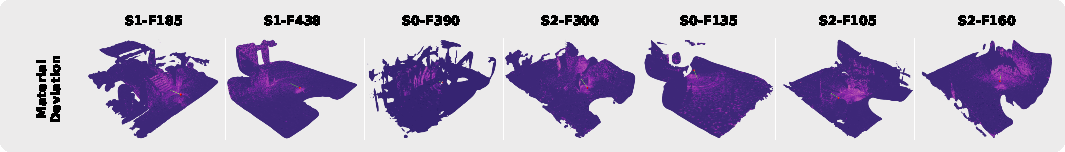
\includegraphics[width=\linewidth]{figs/materials_deviation_v1.pdf}
  \caption{Per-vertex material deviation from ITU-R P.2040 concrete defaults after optimization, shown across all seven scenes. Color encodes the normalized mean deviation across six physics parameters ($\varepsilon_r$, $\varepsilon_i$, $\sigma_h$, $\ell_c$, $\tau$, $d$) using the inferno colormap, where black = zero deviation (unchanged from defaults) and bright yellow = maximum deviation within each parameter's physical range. Log-scale parameters ($\varepsilon_i$, $\sigma_h$, $\ell_c$, $d$) are normalized in log-space; linear parameters ($\varepsilon_r$, $\tau$) in linear-space. Deviations concentrate on radar-visible surfaces and diminish in occluded or shadow regions.}
  \label{fig:3d_material}
\end{figure}

As shown in Fig.~\ref{fig:3d_material}, material deviations are
spatially correlated with radar visibility: surfaces under direct
illumination show the largest updates, while occluded regions retain
their ITU defaults. This pattern is consistent across all seven scenes
despite varying geometry and viewpoints.

\subsection{Surface Normal Visualization}
\label{sec:qual_normals}

\begin{figure}[t]
  \centering
  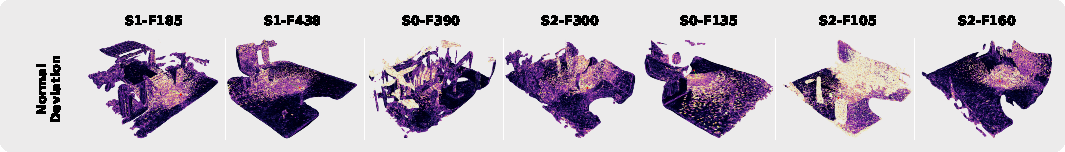
\includegraphics[width=\linewidth]{figs/normals_deviation_v1.pdf}
  \caption{Per-vertex angular deviation between initial (LiDAR-derived) and optimized surface normals across all seven scenes. Color encodes the absolute angle between initial and optimized normal vectors using the inferno colormap, where black = $0^{\circ}$ (no change) and bright yellow = $30^{\circ}$ or greater (clamped at $30^{\circ}$). Larger deviations appear primarily at mesh boundaries and on surfaces with irregular tessellation.}
  \label{fig:normals_deviation}
\end{figure}

\begin{figure}[t]
  \centering
  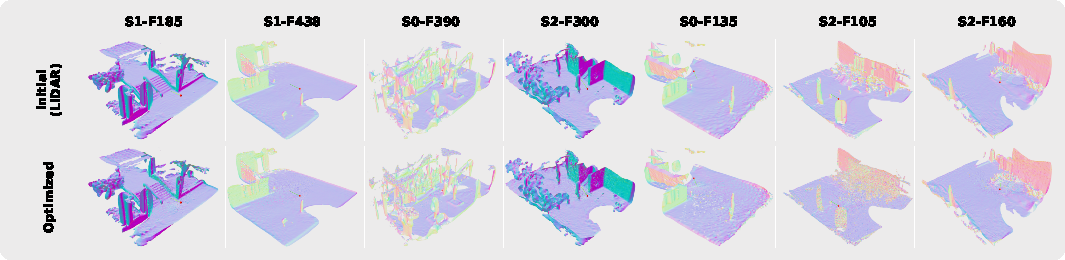
\includegraphics[width=\linewidth]{figs/normals_comparison_v1.pdf}
  \caption{World-space surface normal comparison across all seven scenes. Each vertex is colored by its unit normal direction mapped to RGB (X$\to$R, Y$\to$G, Z$\to$B; value range $[-1,1] \to [0,1]$). Top row (``Initial''): normals computed from the Poisson-reconstructed LiDAR mesh. Bottom row (``Optimized''): normals after joint optimization. Differences between rows show where surface orientations changed during optimization; changes are most apparent at mesh boundaries and on large planar surfaces where Poisson reconstruction artifacts are common.}
  \label{fig:normals}
\end{figure}

Figure~\ref{fig:normals_deviation} shows that angular deviations are spatially concentrated at mesh boundaries, thin structures, and regions with irregular tessellation, all of which are known failure modes of Poisson surface reconstruction from sparse LiDAR returns. Mean angular deviations range from $4^{\circ}$ to $13^{\circ}$ across the seven scenes. Figure~\ref{fig:normals} provides the corresponding world-space normal comparison: large planar regions (walls, ground) remain largely unchanged, while edges and thin features show visible reorientation. This spatial pattern indicates that normal optimization corrects tessellation artifacts rather than overfitting to measurement noise.

\subsection{Antenna Beam Pattern Visualization}
\label{sec:qual_beam}

\begin{figure}[t]
  \centering
  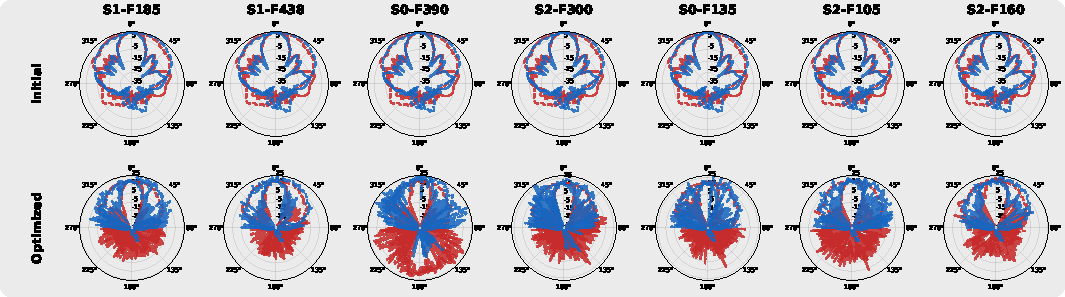
\includegraphics[width=\linewidth]{figs/beam_patterns_comparison_v1.pdf}
  \caption{Antenna beam pattern comparison across all seven scenes (polar plots, dB scale). Each plot shows four curves: TX elevation (red solid), TX azimuth (red dashed), RX elevation (blue solid), and RX azimuth (blue dashed). Top row (``Initial''): reference patterns shared across all scenes. Bottom row (``Optimized''): per-scene optimized patterns. Optimization adjusts main-lobe gain and sidelobe structure to compensate for calibration uncertainty in the reference antenna data. Per-scene variation in the optimized patterns is expected, as each scene compensates independently for calibration uncertainty. All values floored at the initial pattern minimum ($-32$\,dB).}
  \label{fig:beam_patterns}
\end{figure}

As shown in Fig.~\ref{fig:beam_patterns}, the optimized beam patterns retain the main-lobe beamwidths of the initial reference patterns for both TX and RX elements across elevation and azimuth, while adjusting absolute gain levels. Per-scene variation in the optimized patterns reflects independent compensation for calibration uncertainty. The consistent preservation of main-lobe structure across all seven scenes supports the interpretation that pattern optimization primarily refines gain calibration rather than learning physically implausible beam~shapes.


\FloatBarrier
\subsection{Ablation Studies}
\label{sec:ablation}

\begin{table}[ht!]
\caption{Component ablation averaged over seven training scenes (500
iterations each). Each row disables one component from the full mmIR
model. Best per-column in \textbf{bold}.}
\centering
\begin{tabular}{lcccc}
\toprule
\textbf{Configuration} & \textbf{Corr $\uparrow$} & \textbf{PSNR $\uparrow$} & \textbf{SSIM $\uparrow$} & \textbf{RMSE $\downarrow$} \\
\midrule
Full model              & 0.919 & 37.6 & 0.902 & 0.014 \\
\midrule
w/o diffraction         & 0.910 & 37.4 & 0.896 & 0.014 \\
w/o SMS                 & 0.915 & 37.8 & 0.898 & 0.014 \\
w/o multi-bounce        & \textbf{0.936} & \textbf{38.7} & \textbf{0.920} & \textbf{0.012} \\
w/o normal optim.       & 0.919 & 37.4 & 0.909 & 0.014 \\
w/o pattern optim.      & 0.885 & 36.6 & 0.882 & 0.015 \\
w/o error-map init      & 0.909 & 37.4 & 0.895 & 0.014 \\
\bottomrule
\end{tabular}
\label{tab:ablation}
\end{table}


We ablate each component by disabling it from the full model and
retraining on all seven scenes for 500 iterations
(Table~\ref{tab:ablation}). We group ablations into three categories:
rendering transport, optimization targets, and initialization.

\paragraph{Rendering transport.}
Disabling \emph{diffraction} degrades RA correlation ($0.919 \to 0.910$, $-1.0\%$), indicating that edge-diffracted energy
contributes in outdoor scenes with building edges, fences,
and vehicle contours.
%
Disabling \emph{SMS} has a marginal effect on RA metrics
($0.919 \to 0.915$), consistent with the predominantly rough surface
scattering expected at 77\,GHz for outdoor building materials;
SMS primarily benefits scenes with smooth metallic
surfaces (e.g., vehicle panels), which constitute a small fraction of
the total scattering area.
%
Restricting propagation to \emph{single-bounce} slightly improves RA
correlation ($0.919 \to 0.936$) and RMSE
($0.014 \to 0.012$). This suggests that higher-order bounces
introduce Monte Carlo variance at the current sample budget that
slightly degrades metrics, though indirect paths (e.g., ground--wall or
wall--vehicle interactions) contribute measurable energy in the
captured data.

\paragraph{Optimization targets.}
Disabling \emph{antenna pattern optimization} reduces PSNR by
1.0\,dB ($37.6 \to 36.6$) and degrades RA correlation
($0.919 \to 0.885$, $-3.7\%$), indicating that jointly learning beam patterns
compensates for calibration uncertainty in the initial reference antenna
data. As shown in Fig.~\ref{fig:beam_patterns}, the optimized patterns
retain the main-lobe structure and beamwidths of the initial reference
patterns for both TX and RX elements across elevation and azimuth,
indicating that optimization refines gain calibration while preserving
the physical beam structure. The consistent main-lobe preservation
across all seven scenes is consistent with the observation that
disabling pattern optimization primarily degrades PSNR (absolute power
calibration) rather than correlation (spatial structure).
%
Freezing \emph{surface normals} at their LiDAR-derived values has
negligible effect on RA correlation ($0.919 \to 0.919$), while slightly
improving SSIM ($0.902 \to 0.909$). As visualized in
Figs.~\ref{fig:normals_deviation} and~\ref{fig:normals}, normal
optimization concentrates adjustments at mesh boundaries and thin
structures (known failure modes of Poisson surface
reconstruction), with mean angular deviation of $4$--$13^{\circ}$
across scenes, while leaving large planar regions largely unchanged.
This spatial pattern suggests that normal optimization targets
tessellation artifacts rather than overfitting to measurement noise.

\paragraph{Initialization.}
Disabling \emph{error-map initialization} has marginal effect on
final metrics ($0.919 \to 0.909$), indicating that 500 gradient
iterations are sufficient to largely recover from uniform material
initialization. The benefit of error-map seeding is faster early
convergence rather than improved final quality.

\FloatBarrier
\subsection{Runtime}
\label{sec:runtime}

Table~\ref{tab:runtime} reports the runtime breakdown for our pipeline and the Sionna-RT baseline on scene S0F135 ($\sim$72K vertices) using a single NVIDIA RTX 4090 GPU (24\,GB).
Per-scene preprocessing---LiDAR aggregation, Poisson meshing, and radar--LiDAR alignment---is a one-time cost shared by both methods.
During training, our forward render averages 0.65\,s per iteration, roughly $4.5\times$ faster than Sionna-RT's 2.93\,s, owing to our Taichi-based SBR kernel and cached specular-path reuse.
The AD backward pass adds only 0.10\,s.
Including gradient clipping, the Adam optimizer step, and metric computation, the total per-iteration cost is 1.32\,s, enabling 500 iterations in $\sim$11\,min wall-clock time.
At inference, rendering the full dense virtual array (10,000 elements) and computing the RAE FFT takes 6.4\,s per scene.

\begin{table}[ht!]
\centering
\caption{Runtime comparison and breakdown on a single NVIDIA RTX 4090 GPU (24\,GB). Training times are averaged over 500 iterations (mmIR) and 150 iterations (Sionna-RT) on scene S0F135 ($\sim$72K vertices), excluding the first 5 iterations (JIT compilation warmup).}
\label{tab:runtime}
\begin{tabular}{lcc}
\toprule
\textbf{Stage} & \textbf{mmIR (Ours)} & \textbf{Sionna-RT} \\
\midrule
\multicolumn{3}{l}{\emph{Per-scene preprocessing (one-time)}} \\
\quad LiDAR aggregation \& meshing & \multicolumn{2}{c}{144\,s} \\
\quad LiDAR--radar alignment & \multicolumn{2}{c}{2.2\,s} \\
\midrule
\multicolumn{3}{l}{\emph{Training (per iteration, mean $\pm$ std)}} \\
\quad Forward render & 0.65\,s & 2.93\,s \\
\quad AD backward + grad.\ extraction & 0.10\,s & 0.35\,s \\
\quad Grad.\ clipping + optimizer + metrics & 0.57\,s & -- \\
\quad Total per iteration & 1.32 $\pm$ 0.02\,s & 3.28 $\pm$ 0.46\,s \\
\midrule
\multicolumn{3}{l}{\emph{Training (total)}} \\
\quad Total wall-clock & 11.0\,min & 8.2\,min \\
\quad Iterations & 500 & 150 \\
\midrule
\multicolumn{3}{l}{\emph{Inference (one-time per scene)}} \\
\quad Dense array ADC rendering & \multicolumn{2}{c}{6.2\,s} \\
\quad RAE FFT + point cloud & \multicolumn{2}{c}{0.2\,s} \\
\bottomrule
\end{tabular}
\end{table}

\section{Limitations}
\label{sec:limitations}

\subsection{Refraction, Absorption, and Sub-surface Scattering}

Currently, mmIR only models propagation in free space between surface interactions, with interfaces handled by a surface BSDF and diffraction. Transmission into volumes (including glass, plastic, drywall among others), internal attenuation, and sub-surface scattering are not simulated. In effect, any refracted component is absorbed at the first interface. This is reasonable for predominantly metallic and high-contrast scenes, but less accurate for semi-transparent or volumetric media. Supporting these effects would require explicit volumetric permittivity and internal transport via Bidirectional Scattering Distribution Functions (BSDFs), which account for both reflection and transmission.

\subsection{Doppler Phase Term for Moving Radar}

Our FMCW model assumes a static radar pose within each frame and attributes phase only to geometric path length. Ego-motion during a chirp burst introduces an additional Doppler phase term that we do not explicitly model. As a result, mmIR is best matched to quasi-static captures; fast platform motion will induce residual phase errors that cannot be fully absorbed by geometry or material calibration without a time-resolved pose model. Incorporating ego-motion would require a TDM-aware motion model that accounts for platform displacement between successive transmit slots.

\subsection{Dynamic Scenes and Objects}

We optimize a single static mesh with static material parameters to render all ADC measurements. Temporally varying objects (including vehicles, people, vibrating structures) are treated as noise and may appear as blurred or ghosted structure in 3D. To the best of our knowledge, the outdoor scenes chosen from the ColoRadar dataset for our experiments do not feature any moving objects. Accounting for dynamic scenes requires per-frame geometry, deformable models, or an explicit separation of static and dynamic components, which is not currently included and left for future work.

\subsection{Multi-bounce Diffraction}

Diffraction is modeled via the free-space diffraction (FSD) BSDF~\cite{steinberg2024fsd} at single-bounce surface interactions, combined with multi-bounce specular/diffuse reflections. Higher-order diffraction chains (edge--edge, edge--surface--edge) and more detailed grazing-angle behavior are not modeled. Extending to multi-bounce diffraction requires preserving Jones-vector transport along diffracted paths, which the FSD BSDF framework naturally supports. Multi-bounce diffraction may contribute additional energy in highly cluttered or strongly shadowed environments that the current single-bounce model does not capture.

\subsection{Amplitude-Only Gradient Signal}
\label{sec:lim_amplitude_only}

As described in Sec.~\ref{sec:phase_sensitivity_loss_landscape}, each ADC sample contains a phase term $\phi \propto d/\lambda$ that is extremely sensitive to path-length changes: at 77\,GHz ($\lambda \approx 4$\,mm), a sub-millimeter displacement induces an $\mathcal{O}(1)$ change in phase, and a half-wavelength shift produces a full $2\pi$ wrap. In our inverse-rendering setting, small parameter updates change individual path lengths by micrometers, flipping phasor contributions between constructive and destructive interference and producing a highly oscillatory, speckle-like loss landscape with narrow local minima spaced at fractions of the wavelength.

Our default training configuration therefore detaches the phase trigonometric terms $\cos(\phi)$ and $\sin(\phi)$ from the AD graph, propagating gradients only through the amplitude $w$ of each phasor contribution (Sec.~\ref{sec:phase_sensitivity_loss_landscape}). While this improves training stability and convergence, it limits the information available to the optimizer: the loss cannot directly drive parameter updates based on path-length discrepancies. In principle, phase gradients carry complementary geometric information that amplitude alone cannot provide. Enabling full phase+amplitude gradients may benefit future work on joint geometry and material optimization, provided the phase gradient noise can be sufficiently mitigated, for instance via larger sample counts, frequency-dependent phase smoothing, or learned gradient scaling.

\subsection{Mesh Quality Bottleneck}

mmIR is bottlenecked by the quality of the LiDAR-derived mesh used as scene geometry. If the Poisson surface reconstruction introduces artifacts (missing surfaces, incorrect topology, or smoothed-out fine structure), the rendered ADC may diverge from the real measurement despite material or pose optimization. Thin structures (fences, poles, foliage) and regions with sparse LiDAR returns are particularly susceptible to reconstruction error, and may produce \emph{phantom reflectors}: mesh triangles that do not correspond to any real-world surface but still contribute spurious radar returns. Our learnable energy gate $A(\boldsymbol{\omega}_t)$ (Eq.~\ref{eq:bsdf_full}) partially mitigates this: optimization can drive $A \to 0$ for phantom triangles by learning high imaginary permittivity or thin-slab resonance, effectively suppressing their reflected energy.

We further employ an error-map-driven material initialization that identifies over-reflecting triangles (where rendered intensity exceeds ground truth) before gradient-based training and pre-adjusts their roughness and permittivity to reduce phantom contributions. Furthermore, LiDAR ($\lambda \sim 900$~nm) and mmWave radar ($\lambda \sim 4$~mm) interact with surfaces at fundamentally different scales: surfaces that produce strong LiDAR returns (e.g., foliage, thin fabric) may be effectively transparent at mmWave frequencies, while surfaces that are specular at mmWave (e.g., rough concrete) scatter diffusely in LiDAR. The mesh therefore includes surfaces with negligible radar cross-section and may miss structures that are radar-visible but LiDAR-dark. Our learnable energy gate partially compensates by suppressing radar-invisible surfaces, but cannot reconstruct geometry absent from the mesh. Nevertheless, these mechanisms cannot recover surfaces that are missing from the mesh entirely. Mitigating this limitation requires either higher-fidelity meshing pipelines (e.g.,\ neural implicit surfaces, multi-frame aggregation) or jointly optimizing coarse mesh topology during inverse rendering.

\subsection{Sensitivity to Sensor Alignment}

The inverse rendering task is highly sensitive to the LiDAR--radar alignment, both for the cascaded imaging radar used during training and the single-chip radar used for transfer evaluation. Small translational or rotational errors shift rendered paths relative to measured ones, introducing systematic phase errors that material optimization alone cannot absorb. Our coarse-to-fine GPU alignment mitigates gross misalignment but may converge to local optima in scenes with ambiguous geometry (flat surfaces, repetitive structure). This sensitivity is amplified for multi-chip cascade configurations where inter-chip calibration errors compound across the virtual array.



% ---------------------------------------------------------------
% Bibliography
\bibliographystyle{splncs04}
\bibliography{main,supplement}

\end{document}
